
\begin{figure*}[!t]
\centering
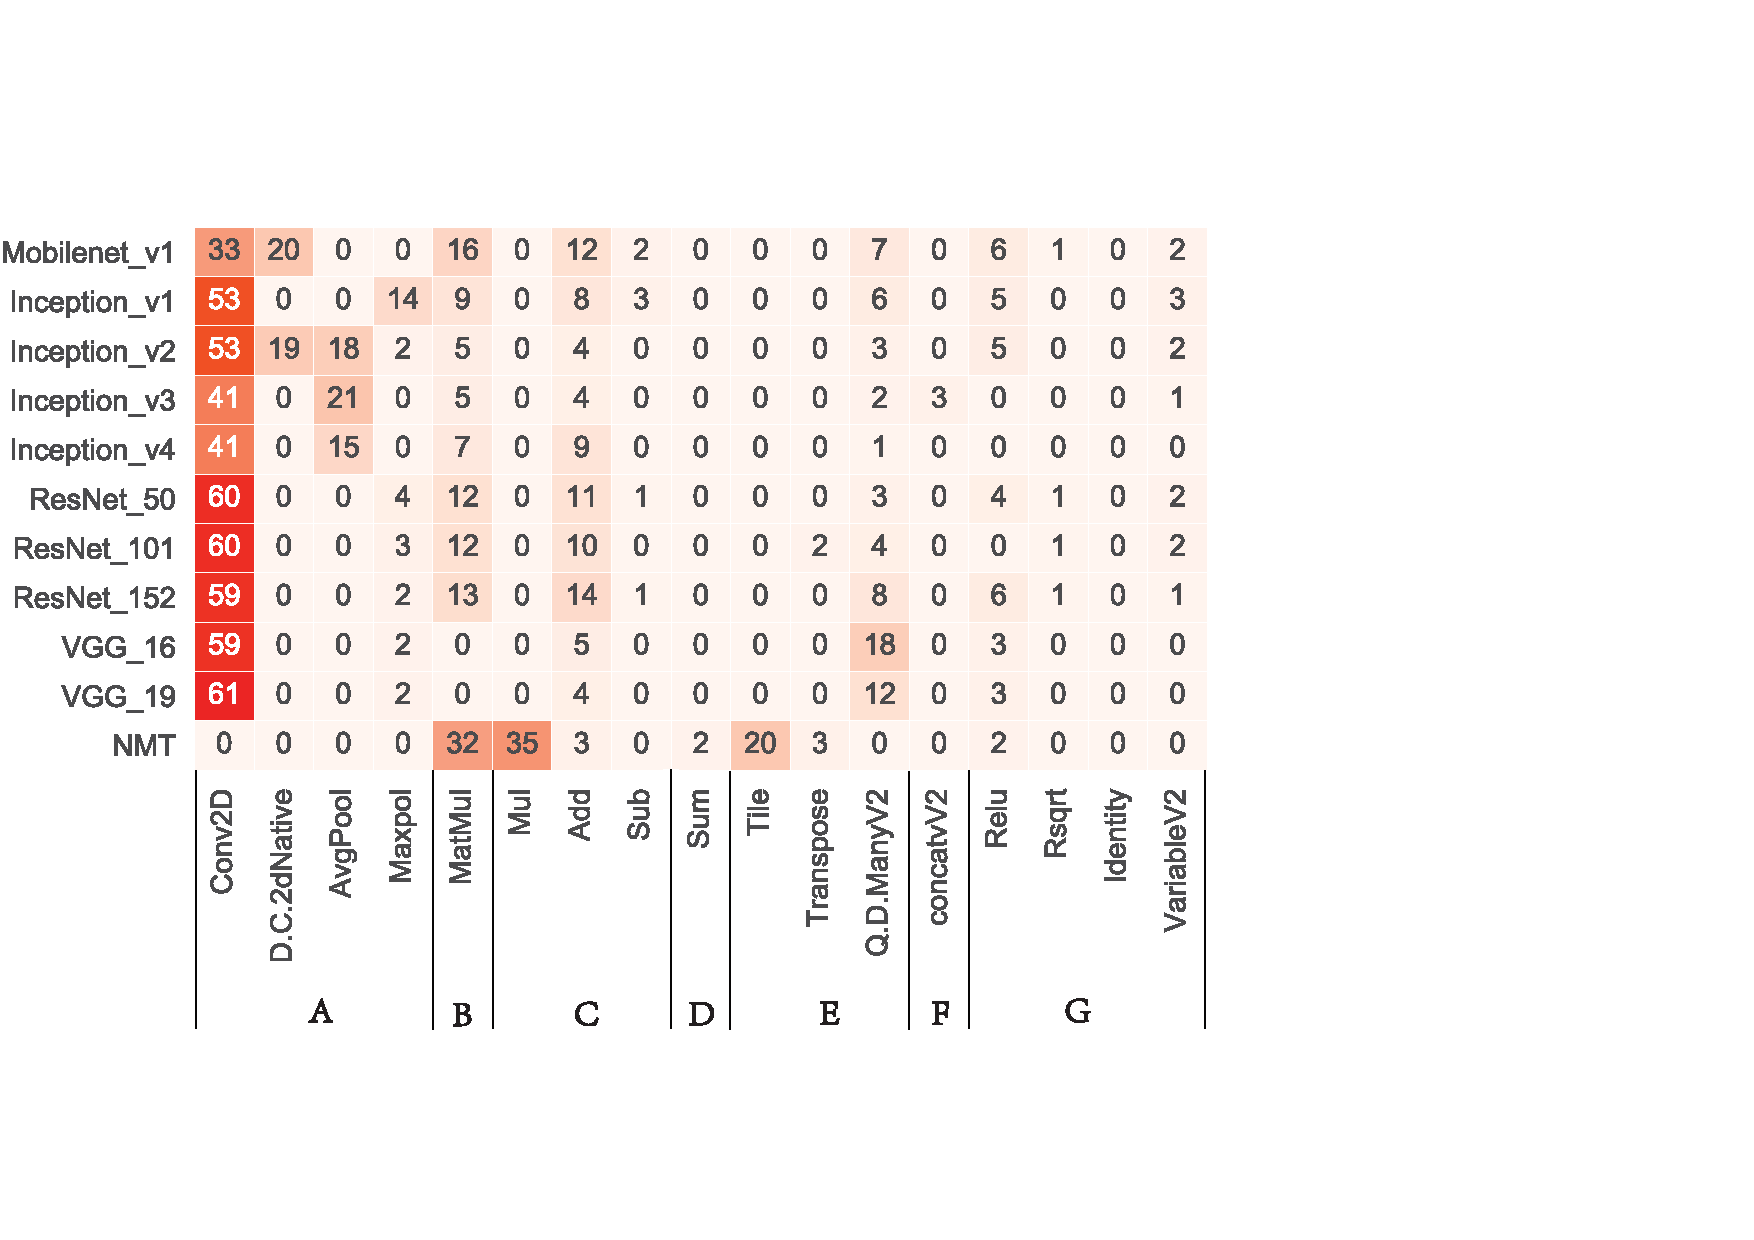
\includegraphics[width=0.7\textwidth]{figure/break11models.pdf}
\caption{ Breakdown of execution time by operation type for every listed models in Table~\ref{tab:workload}.}
 \label{fig:breakdown11}
\end{figure*}

\begin{figure*}[!t]
\centering
\subfloat[][Model size]{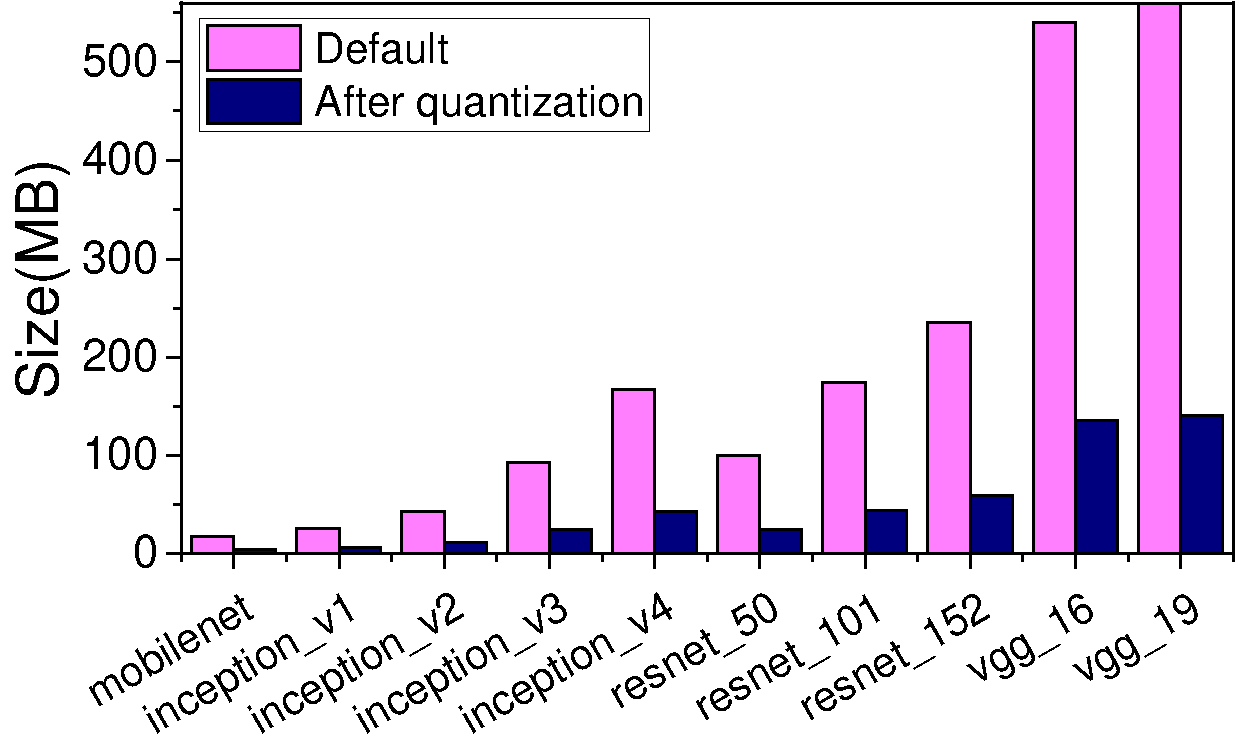
\includegraphics[width=0.33\textwidth]{figure/quan_size.pdf}}
\hfill
\subfloat[][Inference time]{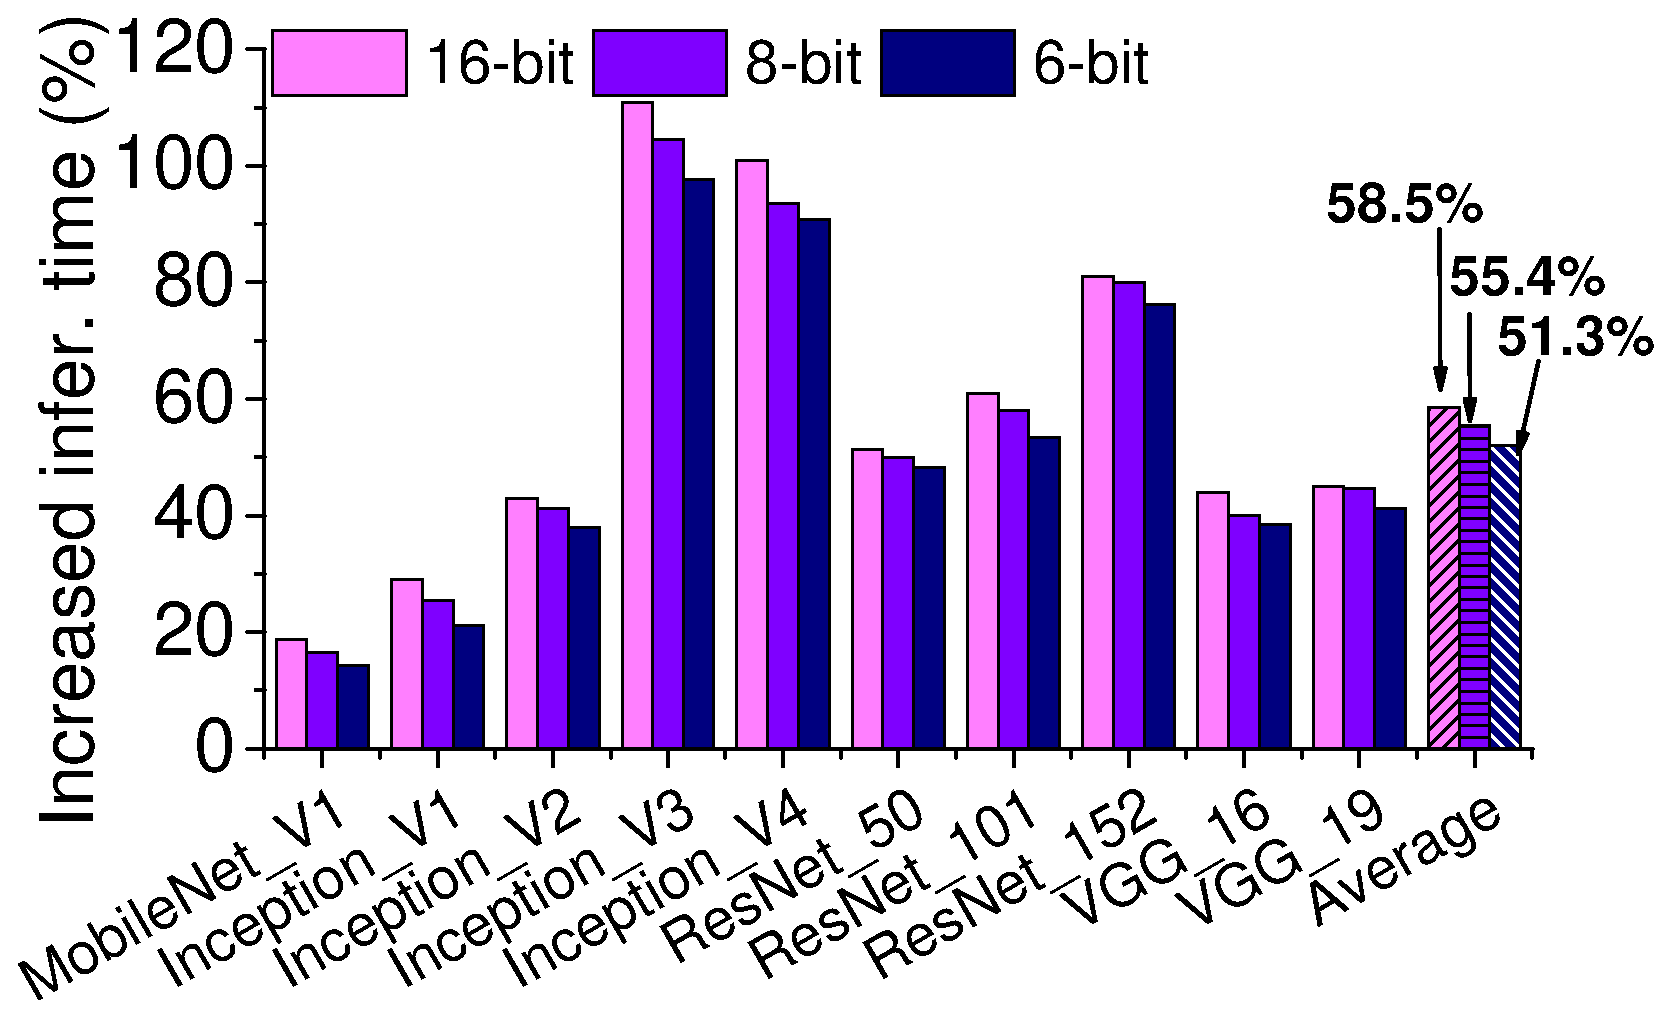
\includegraphics[width=0.34\textwidth]{figure/quan_time2.pdf}}
\hfill
\subfloat[][Accuracy]{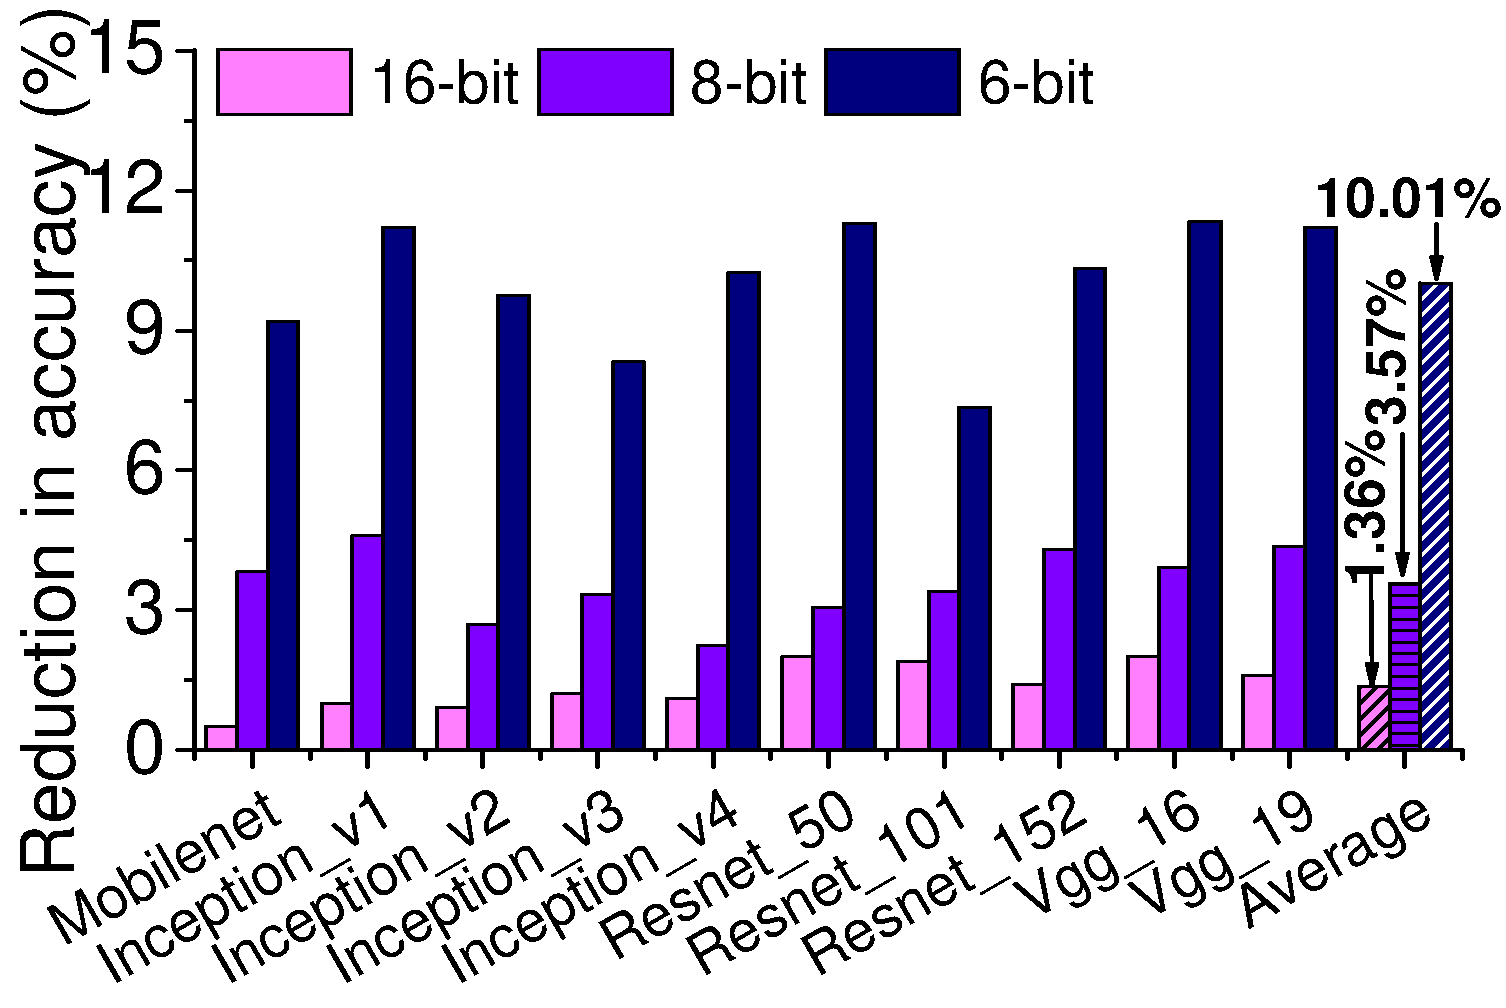
\includegraphics[width=0.32\textwidth]{figure/quan_acc3.pdf}}
\hfill
\subfloat[][Power]{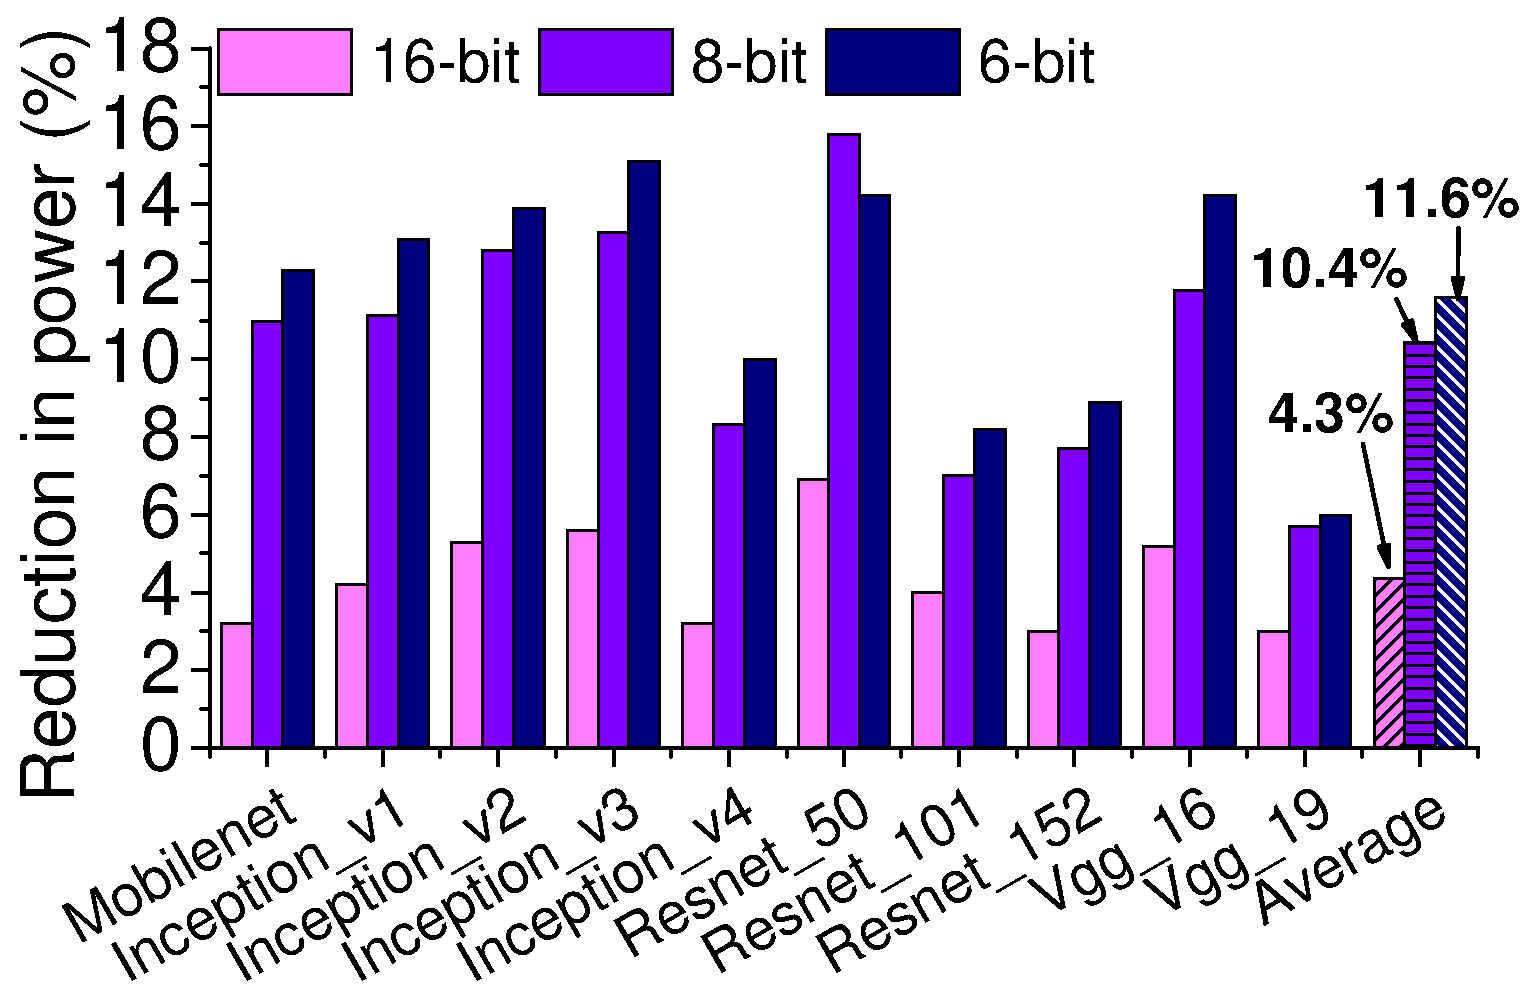
\includegraphics[width=0.33\textwidth]{figure/quan_power2.pdf}}
\hfill
\subfloat[][Energy consumption]{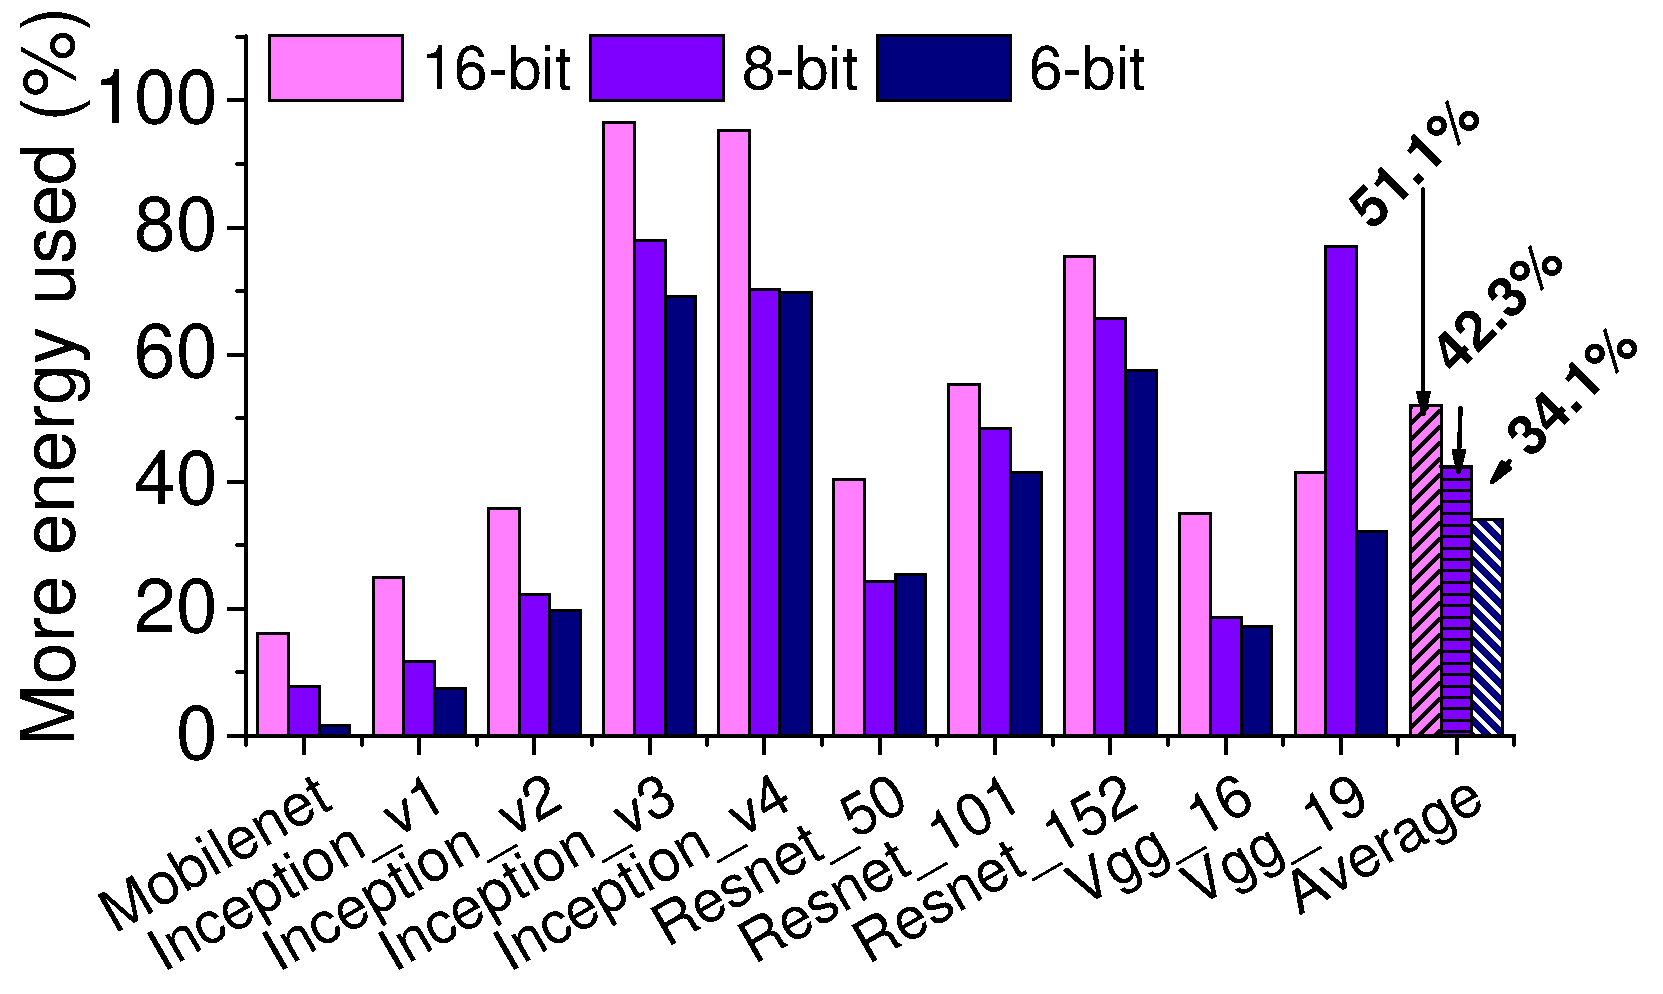
\includegraphics[width=0.34\textwidth]{figure/quan_energy2.pdf}}
\hfill
\subfloat[][Precision, recall and F1-score]{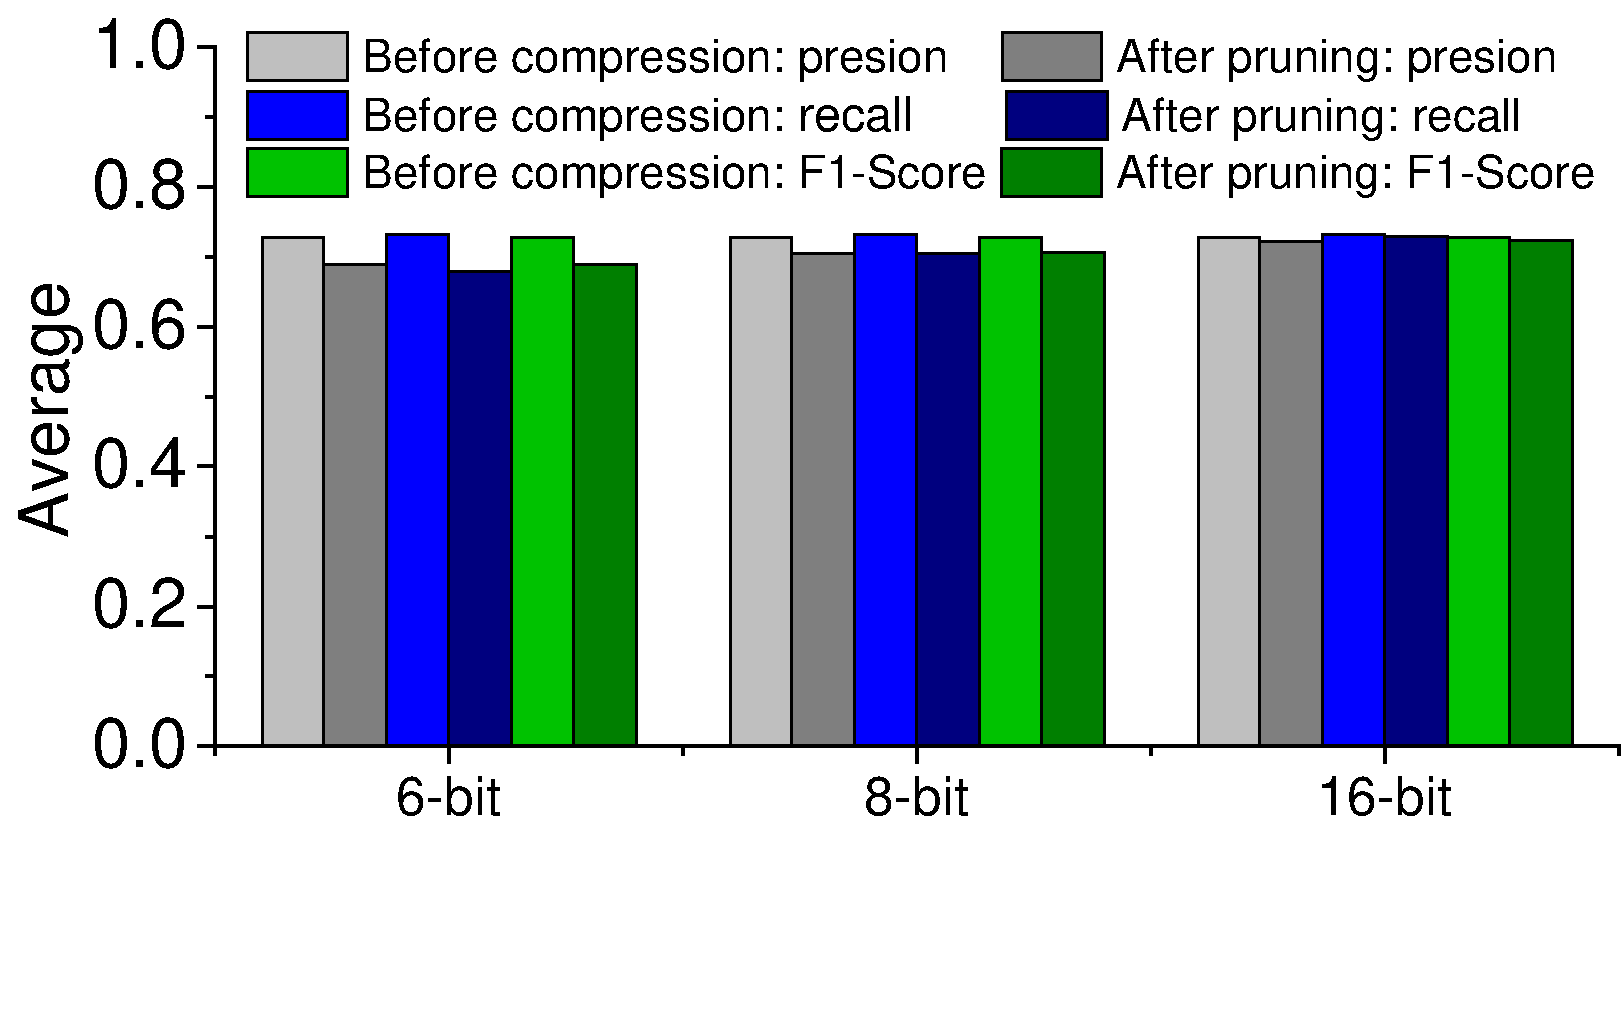
\includegraphics[width=0.33\textwidth]{figure/quan_prf2.pdf}}
\hfill
\caption{The achieved model size (a) inference time (b) accuracy (c) power consumption (d)
energy consumption (e) and precision, recall and F1-score (e) before and after the compression by \quantization.
The compression technique to use depends on the optimization target.}
\label{fig:analy_quan}
\vspace{-3mm}
\end{figure*}

\begin{figure*}[!t]
\centering
\subfloat[][VGG\_16]{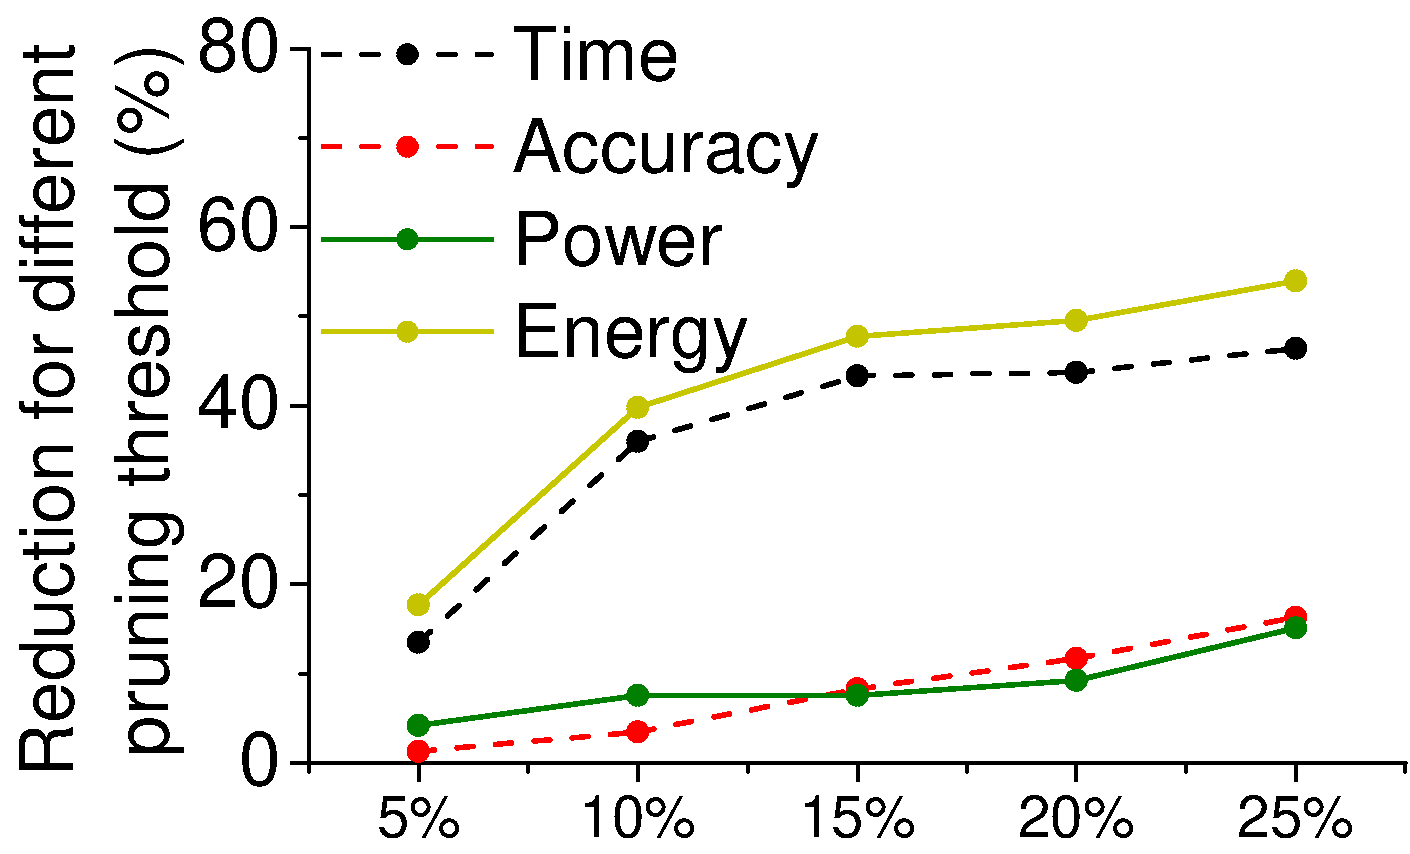
\includegraphics[width=0.3\textwidth]{figure/prun_vgg.pdf}}
\hfill
\subfloat[][ResNet\_50]{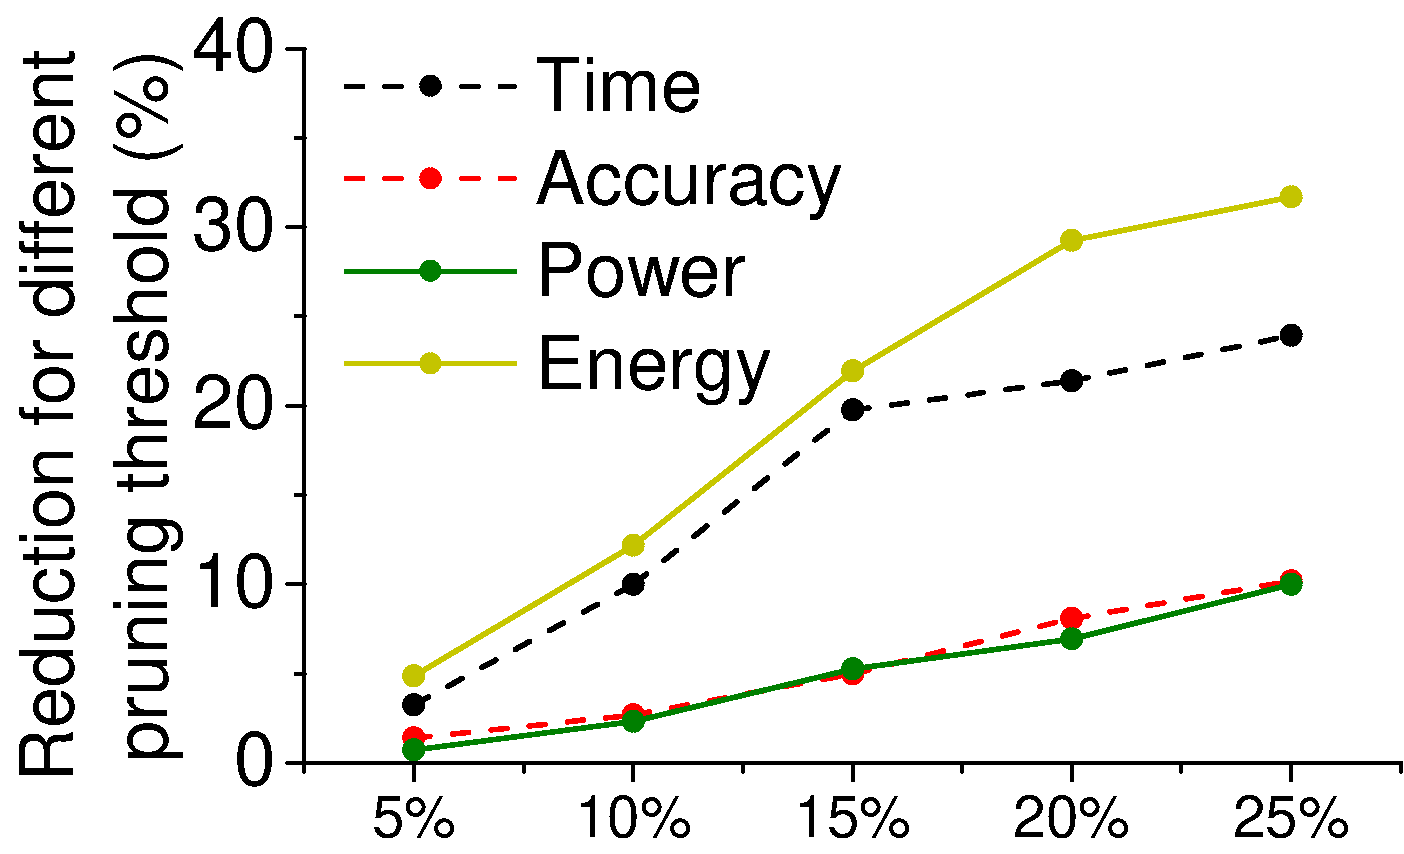
\includegraphics[width=0.3\textwidth]{figure/prun_resnet.pdf}}
\hfill
\subfloat[][NMT]{\includegraphics[width=0.3\textwidth]{figure/prun_NMT.pdf}}
\hfill
\caption{The resulting inference time, accuracy, and power and energy consumption
for Vgg\_16 (a), Resnet\_50 (b) and \texttt{NMT} (c) when using different pruning thresholds.
The x-axis shows the percentage of pruning in model size. }
\label{fig:threshold}
\end{figure*}

\begin{figure*}[!t]
\centering
\subfloat[][Model size]{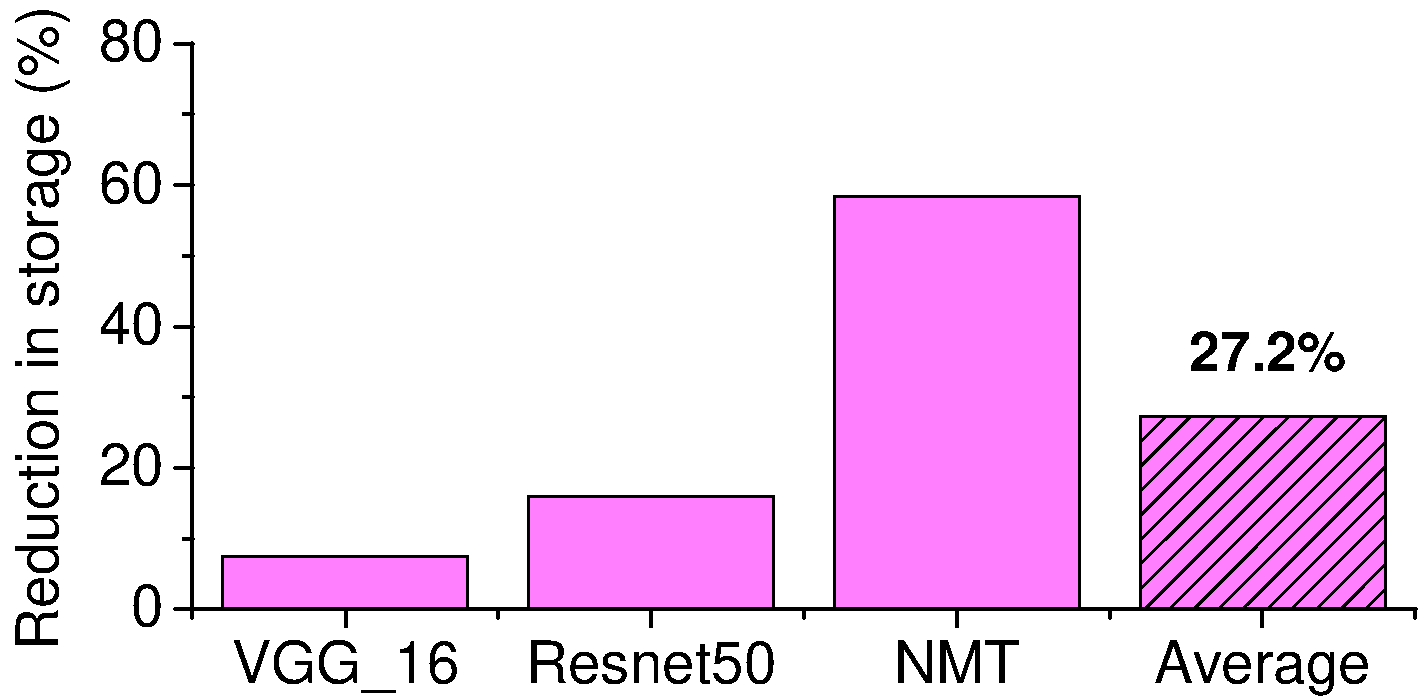
\includegraphics[width=0.33\textwidth]{figure/prun_size.pdf}}
\hfill
\subfloat[][Inference time]{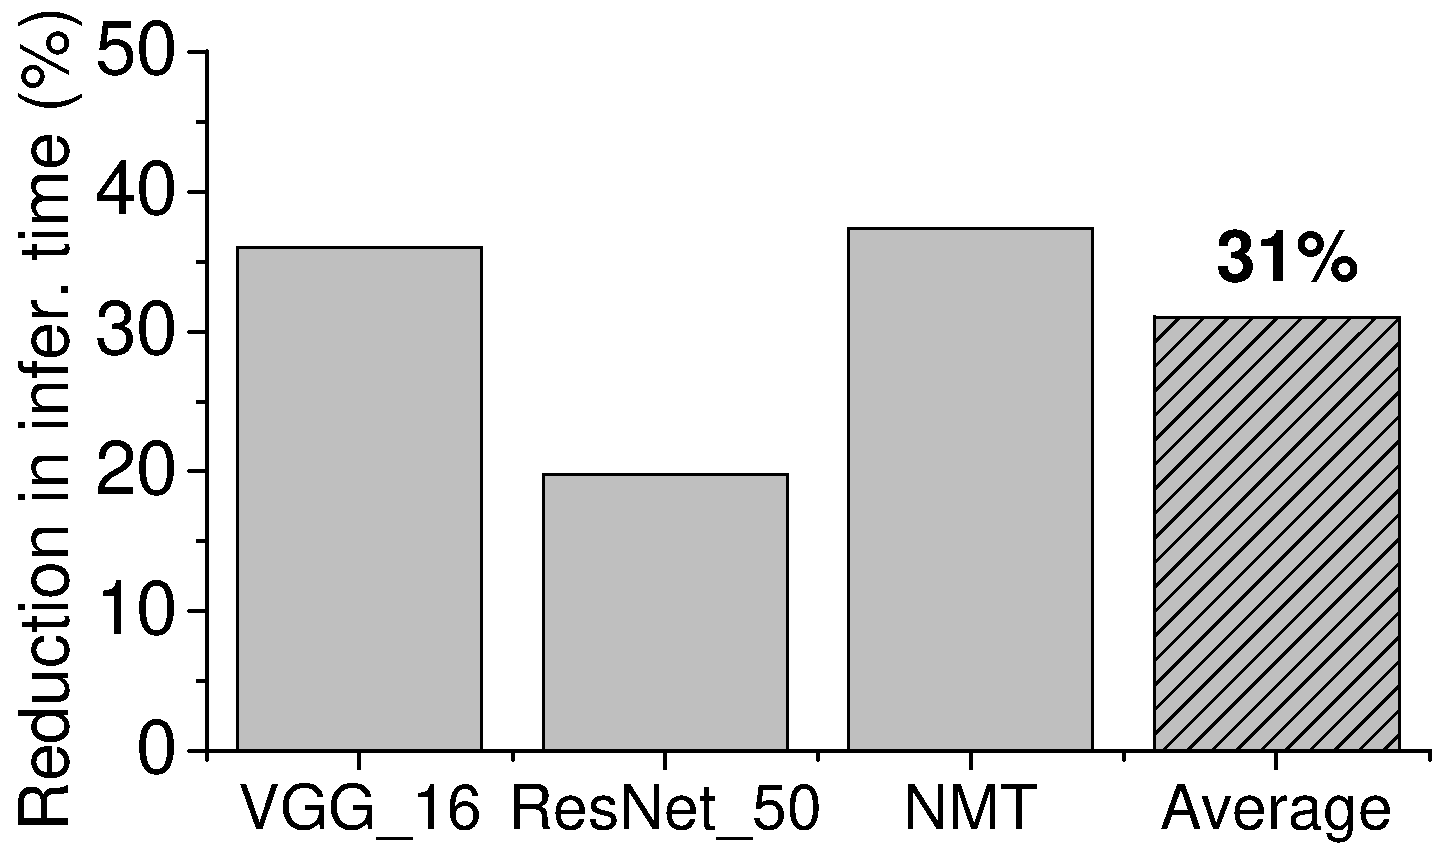
\includegraphics[width=0.3\textwidth]{figure/prun_time.pdf}}
\hfill
\subfloat[][Accuracy]{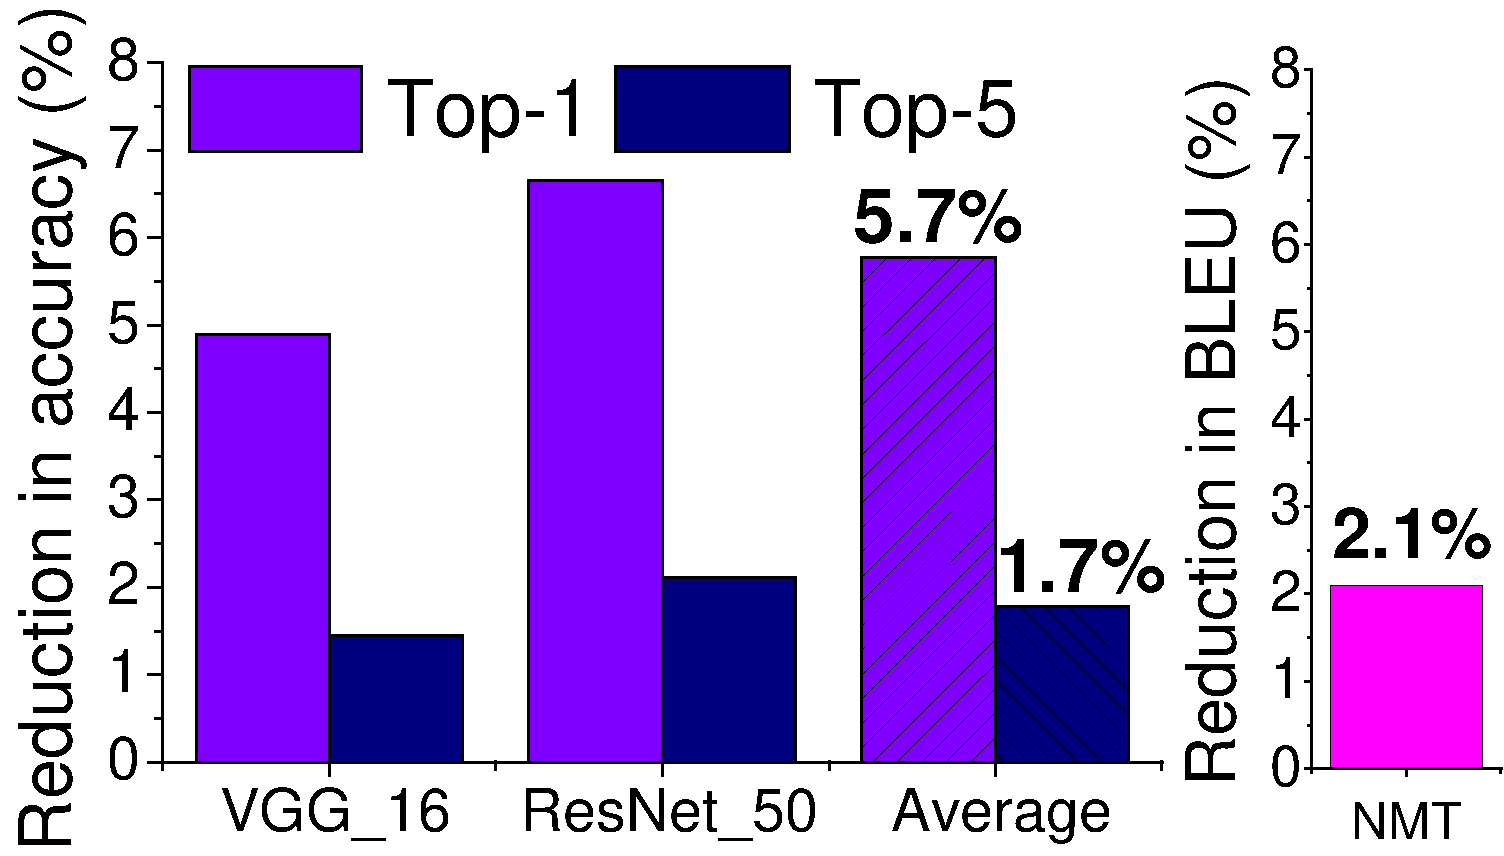
\includegraphics[width=0.3\textwidth]{figure/top1_5_prun.pdf}}
\hfill
\subfloat[][Power consumption]{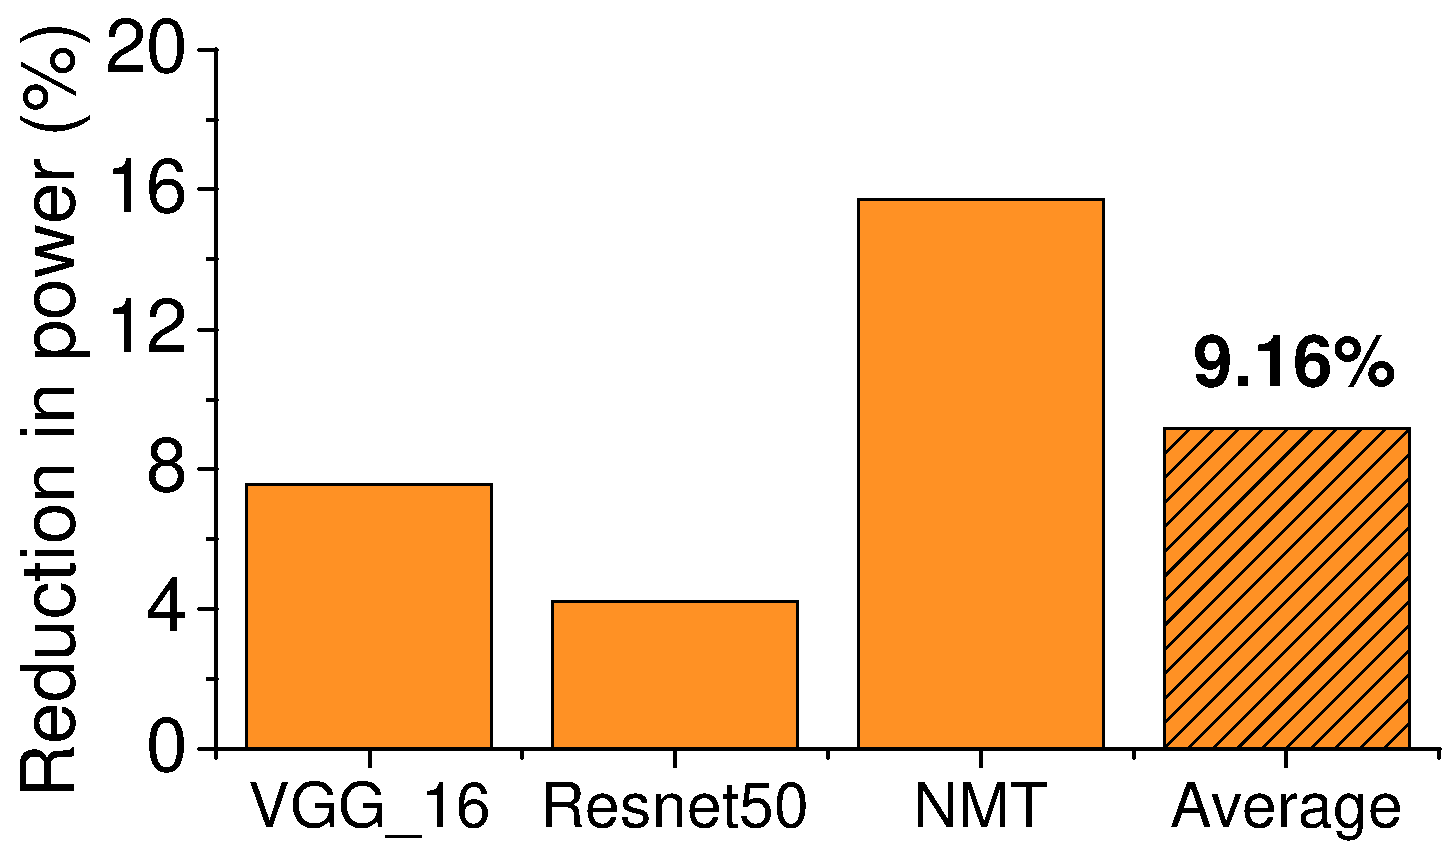
\includegraphics[width=0.3\textwidth]{figure/prun_power.pdf}}
\hfill
\subfloat[][Energy consumption]{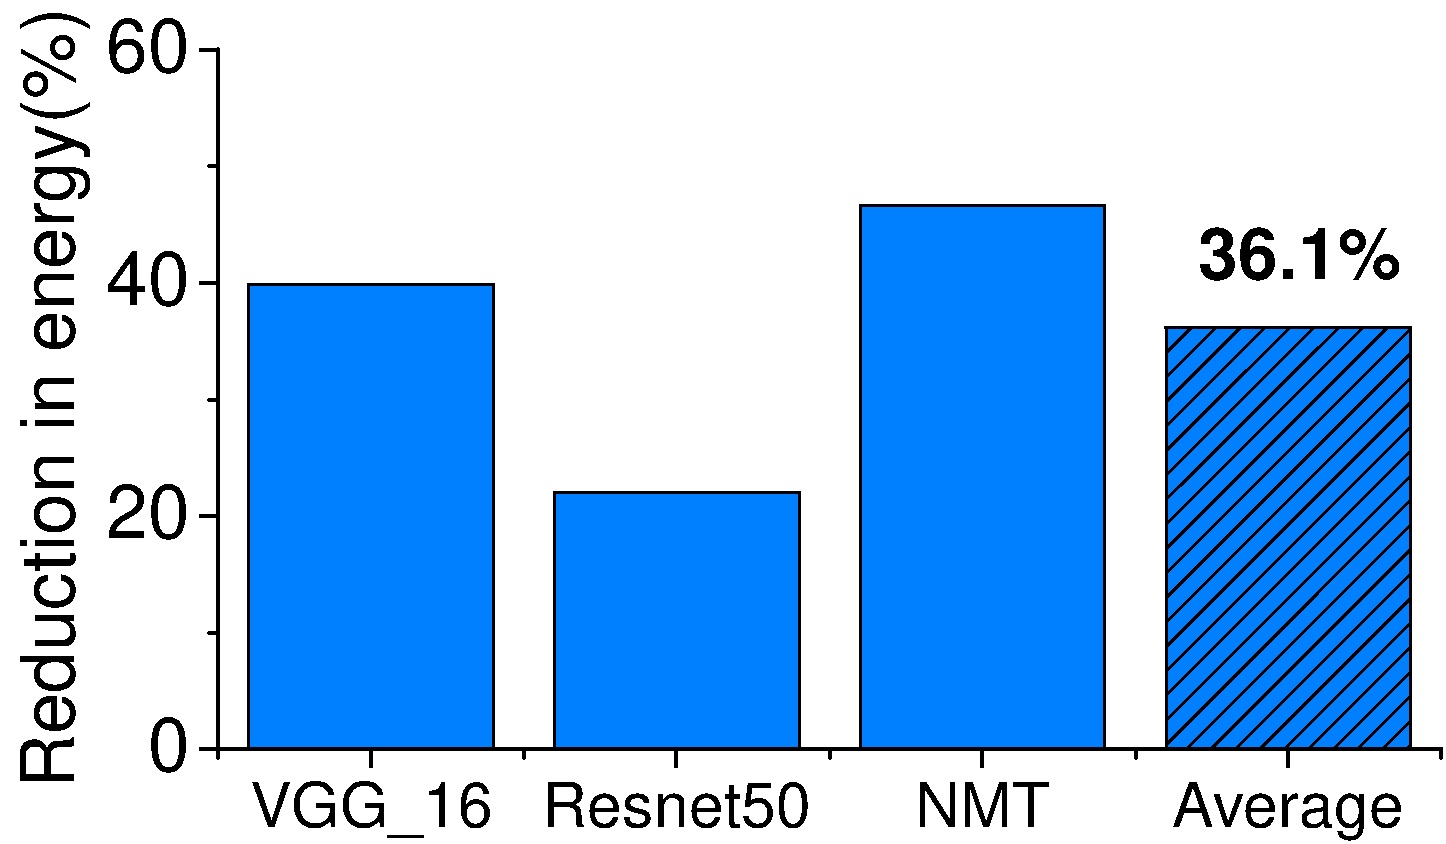
\includegraphics[width=0.3\textwidth]{figure/prun_energy.pdf}}
\hfill
\subfloat[][precision, recall and F1 score]{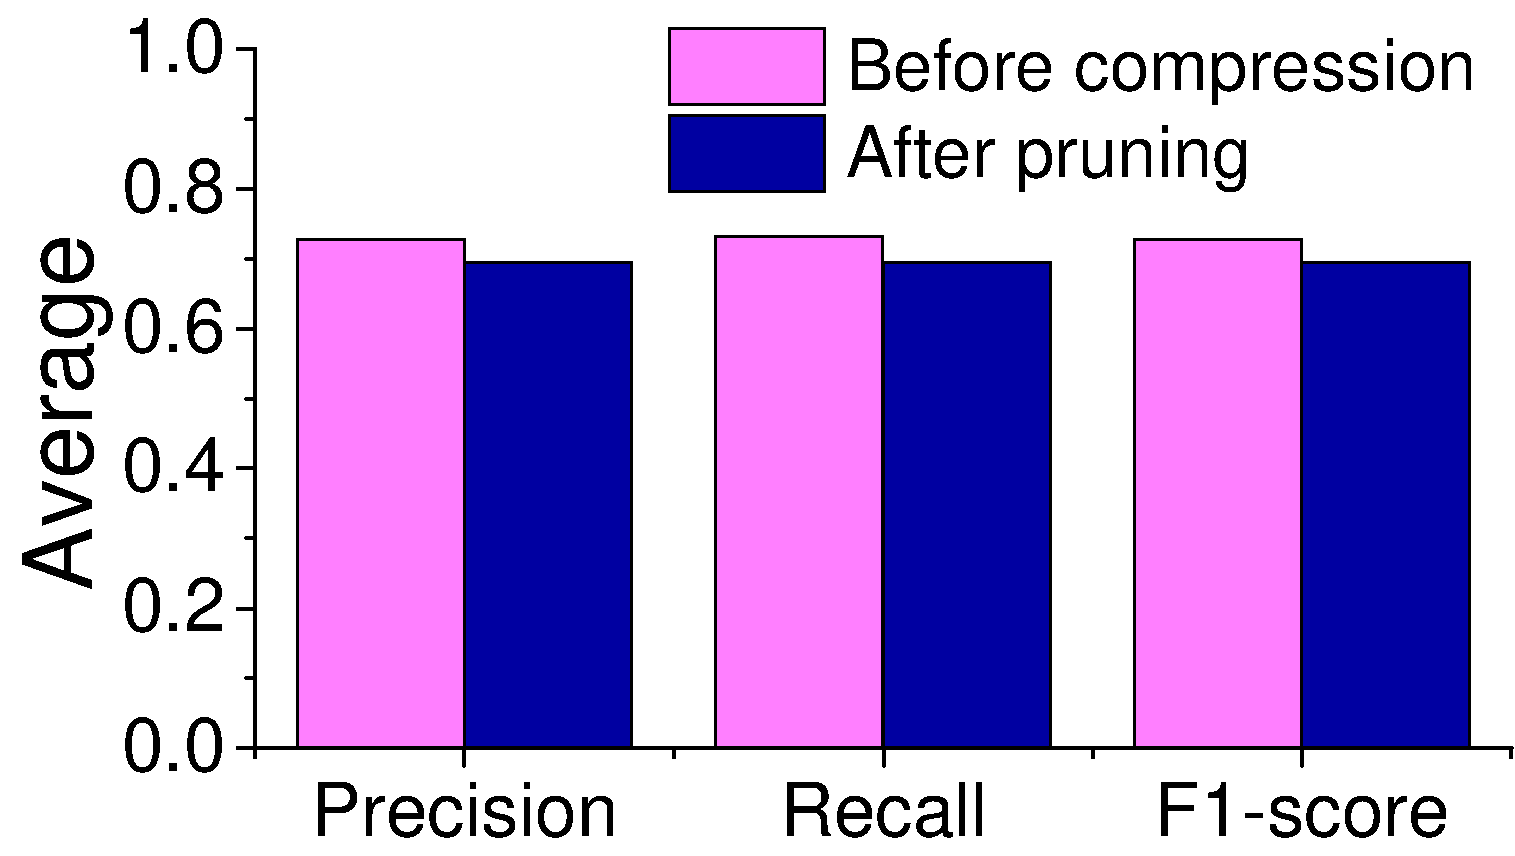
\includegraphics[width=0.3\textwidth]{figure/prun_prf.pdf}}
\hfill
\caption{The change of the model size (a), inference time (b), accuracy/BLEU (c), power (d), energy consumption (e), and accuracy (e)before and after applying \pruning.} \label{fig:analy_prun}
\vspace{-4mm}
\end{figure*}





\section{Experimental Results}


\subsection{Roadmap}
Our experiments try to answer the following questions:

\begin{itemize}
\item How does each compression technique performs across neural network architectures and optimization constraints
    (Sections~\ref{sec:ms} - G)?
\item Is there a ``one-fits-for-all" universal compression technique? (Sections~\ref{sec:single})? If not, what each compression
    technique is good at?
\item Will it beneficial to combine multiple compression techniques (Section~\ref{sec:combin})?
\end{itemize}

\subsection{Operation type profiling}
The general intuition about a handful of operation types dominating the overall computational time is true. While it is
an exaggeration to say that a workload can be reduced to a single operation, the distribution is quite skewed, as shown in
Figure~\ref{fig:breakdown11}. Each point on each curve represents the cumulative
contribution to execution time from a single operation type.
It is clear that a handful of heavy operation types (usually
5 to 15) are collectively responsible for upwards of 90% of
the programs’ duration. It is important to note, however, that
these types are not the same for every model.
Unsurprisingly, convolutional neural networks are indeed
dominated by convolution, and fully-connected networks depend
heavily on matrix multiplication.


\subsection{Impact on the Model Storage Size\label{sec:ms}}
Reducing the model storage size is crucial for embedded and IoT systems which often have a limited storage space. A smaller model size also
translates to smaller runtime memory footprint of less RAM space usage. Figures~\ref{fig:analy_quan},\ref{fig:threshold} and \ref{fig:analy_prun} illustrate
how the different compression techniques and parameters affect the resulting model size.

As can be seen from Figure~\ref{fig:analy_quan}a, data quantization can significantly reduce the model storage size, leading to an average
reduction of 50.2\% when using a 16-bit representation and up to 80.7\% when using a 6-bit representation. The reduction in the storage
size is consistent across neural networks as the size of a network is dominated by its weights.

From Figure~\ref{fig:analy_prun}a, we see that by removing some of the neurons of a network, \pruning can also reduce the model size,
although the gain is smaller than \quantization if we want to keep the accuracy degradation within 5\%. On average, \pruning reduces the
model size by 27.2\% (49.26 MB). An interesting observation is that, \pruning is particularly effective for obtaining a compact model for
\texttt{NMT}, an \RNN, with a reduction of 60\% on the model storage size. This is because there are many repetitive neurons (or cells) in
an \RNN due to the natural of the network architecture. As we will discuss later, \pruning only causes a minor degradation in the
prediction accuracy for \texttt{NMT}. This suggests that \pruning can be an effective compression technique for \RNNs.

In Figure~\ref{fig:threshold}, we compare the resulting performance after using different pruning thresholds from 5\% to 75\% on two \CNN and a \RNN
models. Increasing the pruning percentage of model size does gives \pruning more opportunity to remove more neurons to improve the inference
time and other metrics. The improvement reaches a plateau at 15\% of reduction for \CNNs, but for \texttt{NMT}, a \RNN model, the reduction of
inference time increases as we remove more neurons. This diagram reinforces our findings that \pruning is more effective on \RNNs
than \CNNs. For the rest discussions of this paper, we use a 5\% \pruning threshold.


 %In this paper, we consider the 5\% reductions in the top-1 accuracy is the pruning threshold, and Figure~\ref{fig:threshold}
%present the results when the accuracy around the thresholds.



\subsection{Memory footprint}

\begin{figure}[!t]
\centering
\subfloat[][\quantization]{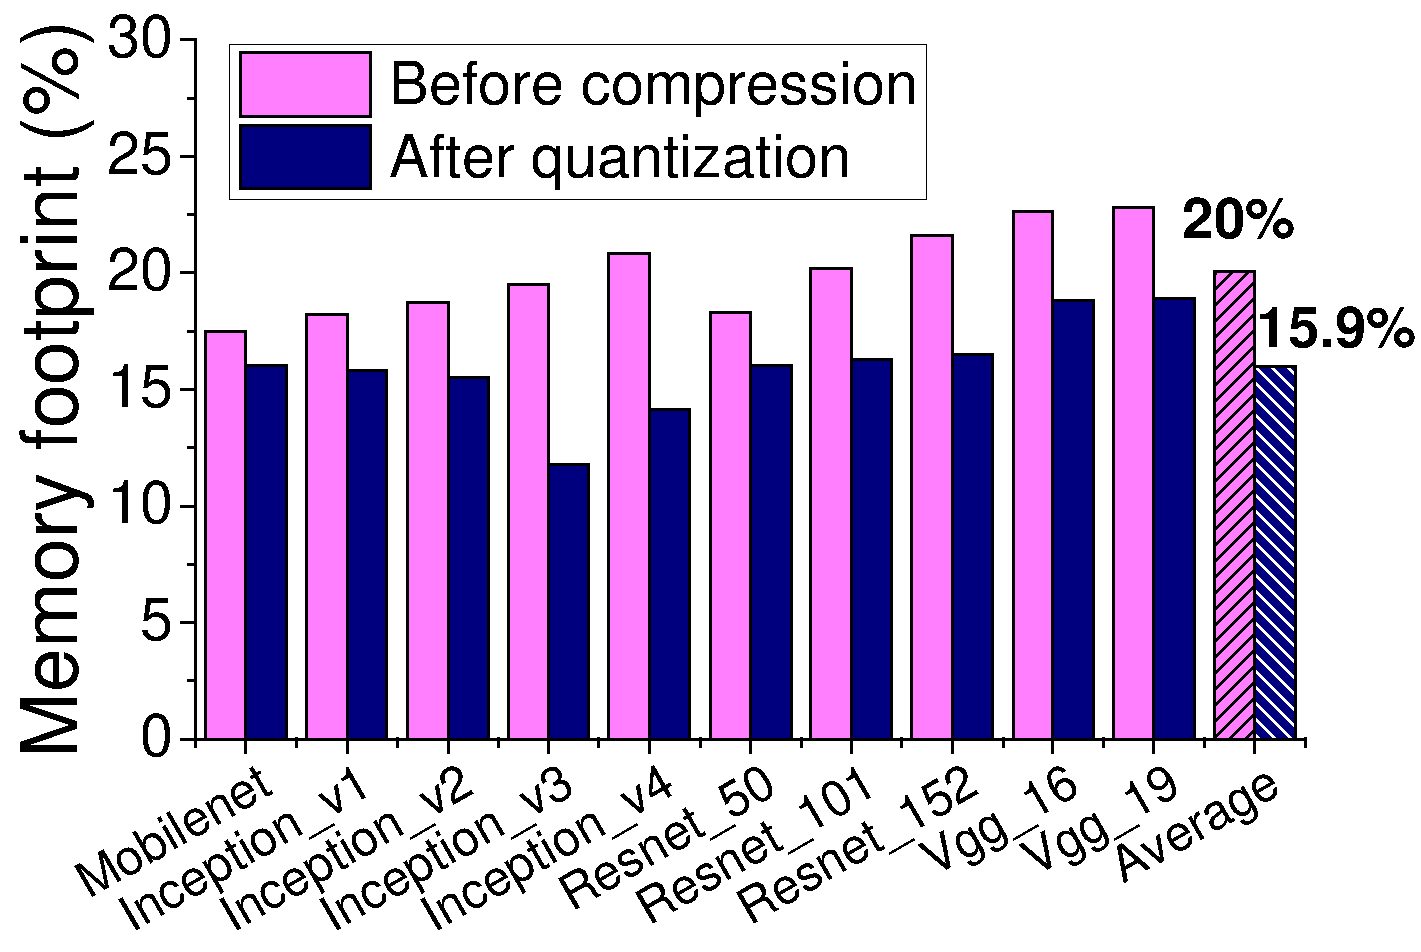
\includegraphics[width=0.4\textwidth]{figure/quan_mem.pdf}}
\hfill
\subfloat[][\pruning]{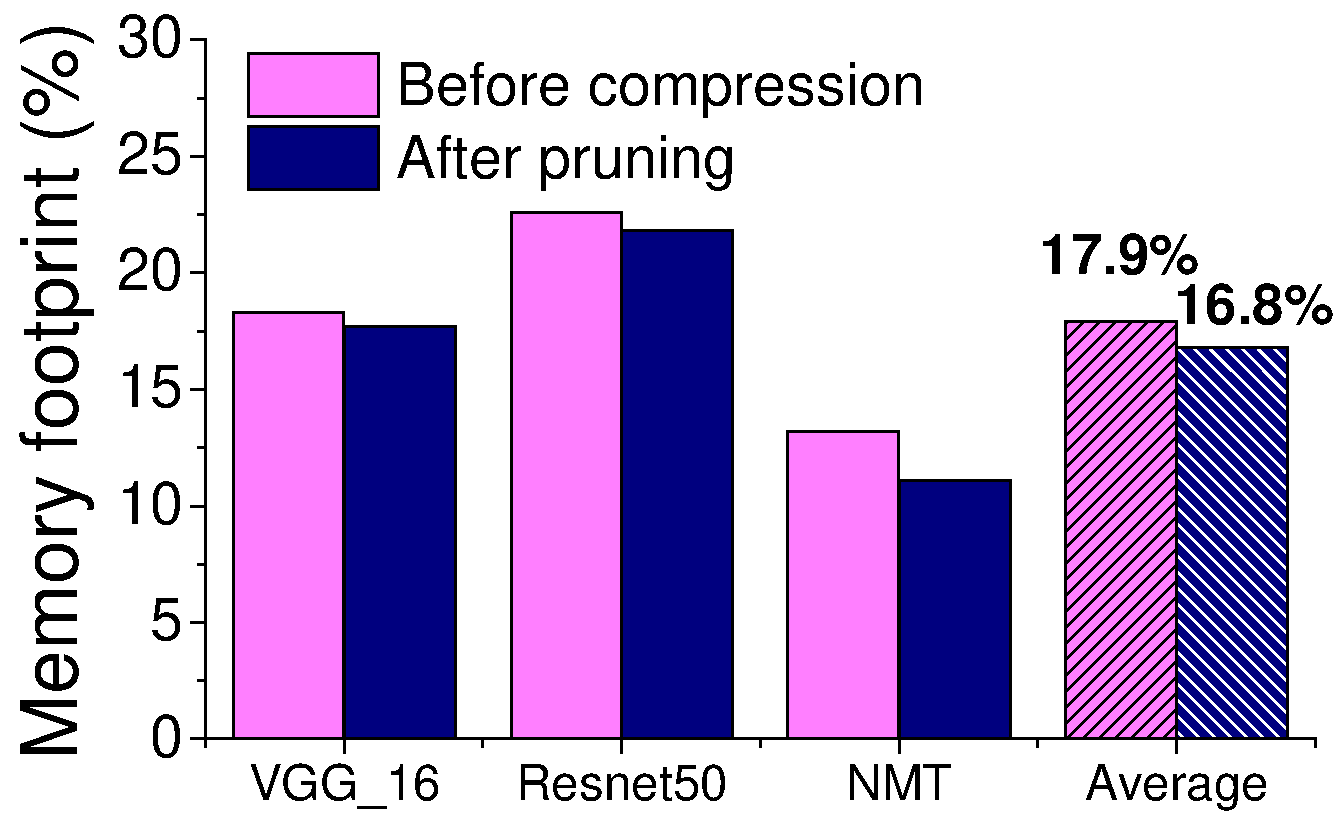
\includegraphics[width=0.39\textwidth]{figure/prun_mem.pdf}}
\hfill

\caption{Memory footprint before and after applying \quantization(a) and \pruning (b).} \label{fig:footprint}
\end{figure}

Figure~\ref{fig:footprint} compares the runtime memory footprint consumed by a compressed model. Quantization reduces the model memory
footprint by 17.2\% on average. For example, an 8-bit representation gives a memory footprint saving from 20.02\% to 15.97\% across
networks, with an averaged reduction of 20.63\% (up to 40\%). In general, the smaller the model storage size is, the less memory footprint
the compressed model will be. As an example, a 6-bit representation uses 2.6\% and 13.6\% less memory compared to an 8-bit and a 16-bit
counterparts, respectively.

Figure~\ref{fig:footprint} suggests that  \pruning offers little help in reducing the model memory footprint. On average, it gives a 6.4\%
reduction of runtime memory footprint. This is because that the network weights still domain the memory resource consumption, and \pruning
is less effective compared to \dquantization for reducing the overhead of network weights.



\subsection{Impact on Inference Time\label{sec:time}}
 Figure~\ref{fig:analy_quan}b compares the inference time when using different bit
widths to represent a 32-bit floating number for neural network weights. Intuitively, a smaller model should run faster. However, data
quantization does not shorten the inference time but prolongs it. The reasons are described as follows. Data quantization can speedup the
computation (i.e., matrix multiplications) performed on some of the input data by avoiding expensive floating point arithmetics and
enabling SIMD vectorization by using a compact data representation. However, we found that the overhead of the de-quantization process
during inference can outweigh its benefit. Besides the general inference operation, a data quantization and de-quantization function has to
be added into the compressed model. Inference performed on a quantized model accounts for 50.9\% of its running time, the de-quantization
functions converts input values back to a 32-bit representation on some of the layers (primarily the output layer) in order to recover the
loss in precision. As can be seen from Figure~\ref{fig:breakdown}, this process could be expensive, contributing to 30\% to 50\% of the end
to end inference time.
%this process could be expensive, contributing to 30\% to 50\% of the end to end inference time.
%After data quantization, a de-quantization function has to be added into the compressed model. This  function converts %the quantized
%weights back to a 32-bit representation on the output layer to recover the loss in precision. As can be seen from %Figure~\ref{fig:breakdown},
%this process could be expensive, contributing to 30\% to 50\% of the end to end inference time.

\begin{figure}
\begin{center}
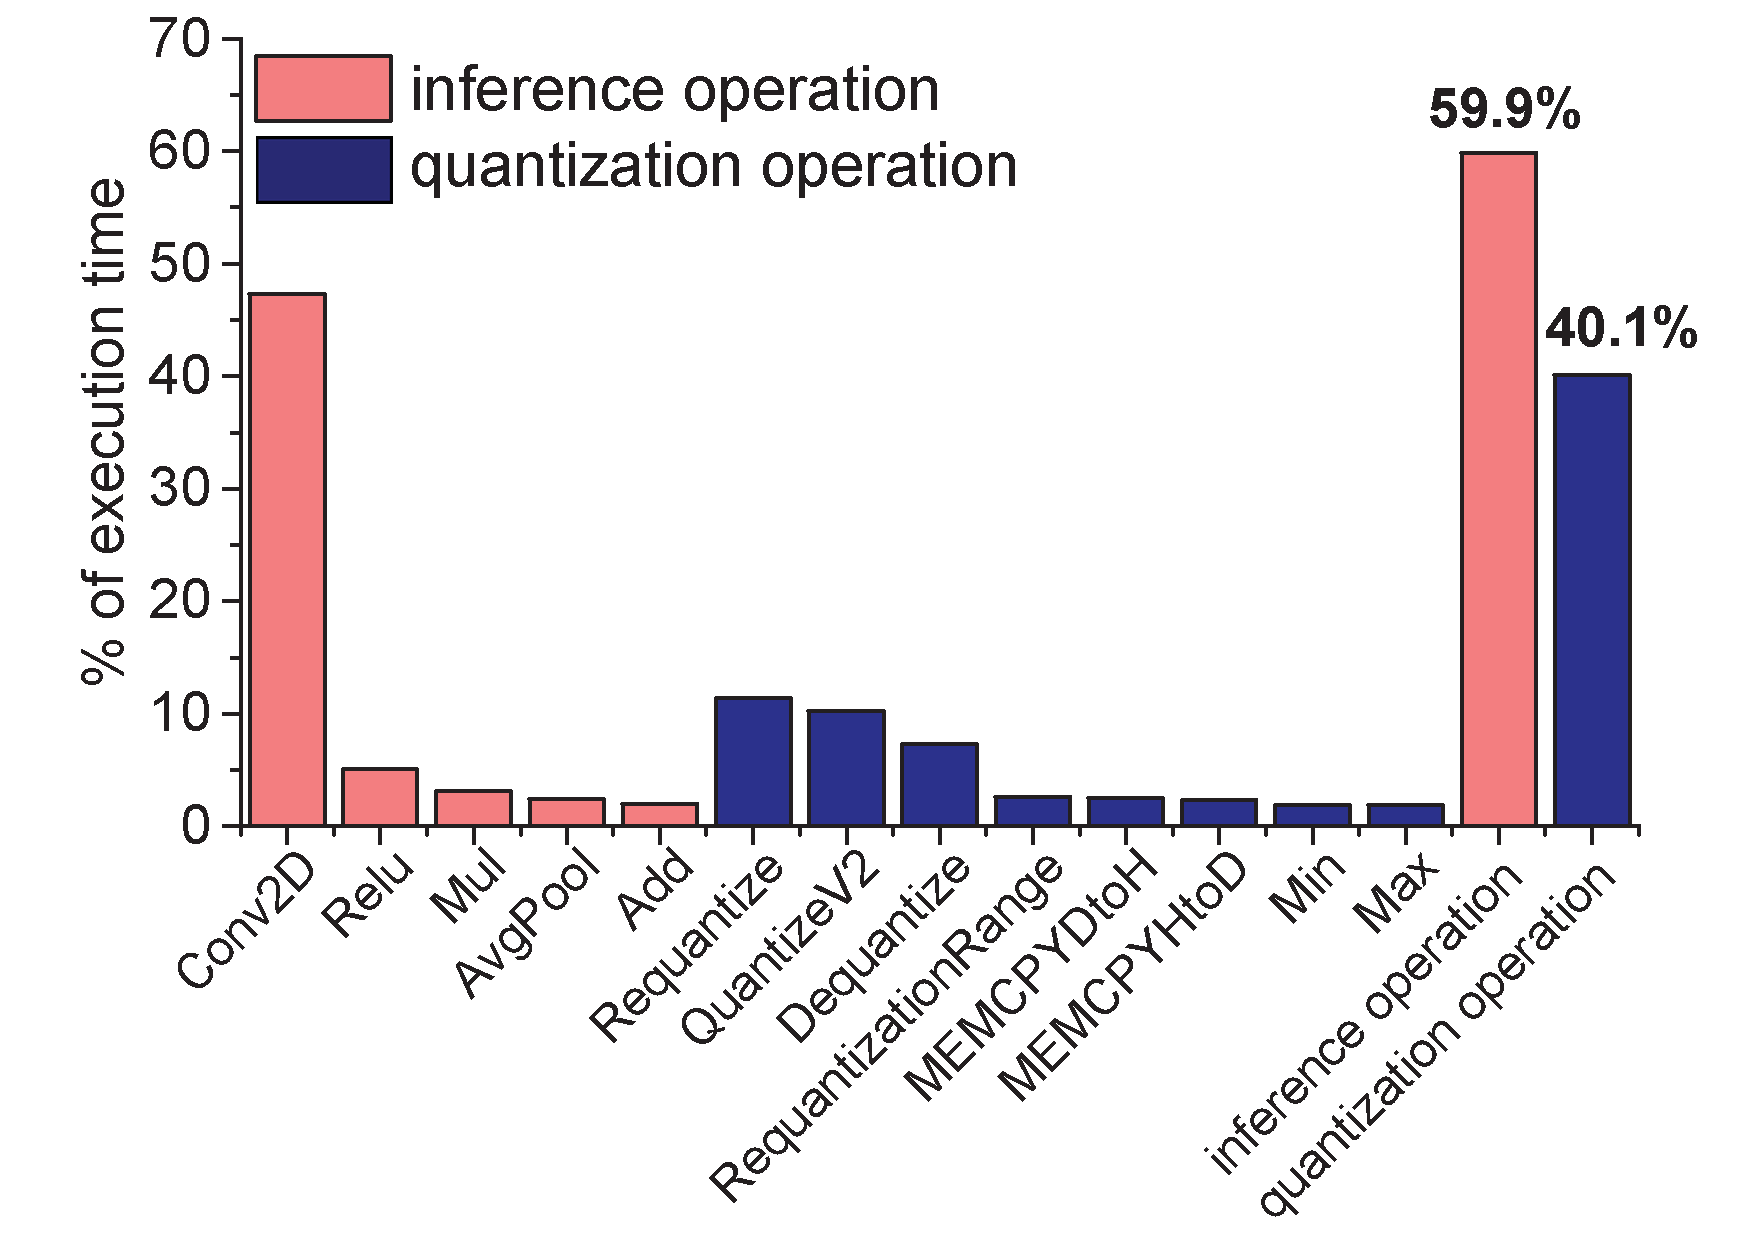
\includegraphics[width=0.4\textwidth]{figure/breakdown4.pdf}
\end{center}
\caption{Breakdown of the average execution time per operation type, averaging across the quantized models.}
\vspace{-3mm}
\label{fig:breakdown}
\end{figure}


Using fewer bits for representation can reduce the overhead of de-quantization. For example, using a 6-bit representation is 1.05x and
1.03x faster than using a 16-bit and a 8-bit representations, respectively. However, as we will demonstrate later when discussing
Figure~\ref{fig:analy_quan}c, using fewer bits has the drawback of causing larger degradation in the prediction accuracy. Hence, one must
carefully find a balance between the storage size, inference time, and prediction accuracy when applying data quantification.

We also find that the percentage of increased inference time depends on the neural network structure. Applying data quantization to
\texttt{Inception}, the most complex network in our \CNN tested set, will double the inference time. By contrast, data quantization only
leads to a 20\% increase in inference time for \texttt{Mobilenet}, a compact model. This observation suggests that data quantization may be
beneficial for simple neural networks on resource-constrained devices.


In contrast to \quantization, Figure~\ref{fig:analy_prun}b shows that \pruning leads to faster inference time across evaluated networks,
because there is no extra overhead added to a pruned network. We see that the inference time of \texttt{Vgg\_16} and \texttt{NMT} can
benefit from this technique, with an reduction of 38\%. Overall, the average inference time is reduced by 31\%. This suggests that while
\pruning is less effective in reducing the model size (see Section~\ref{sec:ms}), it is useful in achieving a faster inference time.

\subsection{Impact on the Power and Energy Consumption}
Power and energy consumption are two limiting factors on battery-powered devices. As we can see from Figure~\ref{fig:analy_prun}d,
\quantization decreases the peak power usage for inferencing with an average value of 4.3\%, 10.4\% and 11.6\%, respectively when using a
6-bit, an 8-bit and a 16-bit representations. While \quantization reduces the peak power the device draws, the increased inference time
leads to more energy consumption (which is a product of inference time $\times$ instantaneous power) by at least 34.1\% and up to 51.1\%
(see Figure~\ref{fig:analy_prun}e). This means that although \quantization allows one to reduces supplied power and voltage, it can lead to
a short battery life.

Figure~\ref{fig:analy_prun}e quantifies the reduced energy consumption by applying \pruning. Note that it saves over 40\%, 15\% and 50\%
energy consumption for \texttt{Vgg\_16}, \texttt{Resne\_50} and \texttt{NMT} respectively. Despite that only minor decreased in the peak
power compared to \quantization (9.16\% vs 34.1\% to 51.1\%), the resulting faster inference time allows \pruning to significantly reduce
the energy consumption. The results suggest \pruning is useful for reducing the overall energy consumption of the system, but \quantization
can be employed to support a low power system.

\subsection{Impact on The Prediction Accuracy}
The accuracy is crucially important for any predictive model. A small and faster model is not useful if it gives wrong predictions all the
time.


Results in Figure~\ref{fig:analy_quan}c compare how the prediction accuracy is affected by model compression. We see that the sweat spot of
\quantization depends on the neural network structure. An 16-bit representation keeps the most information of the original model and thus
leads to little reduction in the prediction accuracy, on average  1.36\%.  Using an 8-bit representation would lead on average 3.57\%
decrease in the accuracy, while using a 6-bit representation will lead to a significantly larger reduction of 10\% in  accuracy. We also
observe that some networks are more robust to \quantization. For example, while a 6-bit representation leads to less than 10\% decrease in
accuracy for \texttt{Resnet\_101}, it cause a 12\% drop in accuracy for \texttt{Resnet\_50}. This is because a more complex network (i.e.,
\texttt{Resnet\_101} in this case) is more resilient to the weight errors compared to a network (i.e., \texttt{Resnet\_50} in this case)
with a smaller number of layers and neurons. Our findings suggest the need for having an adaptive scheme to choose the optimal
\dquantization parameter for given constraints.


For \pruning, Figure~\ref{fig:analy_prun}c compares the reduction in the top-1 and the top-5 scores for \texttt{Vgg\_16} and
\texttt{Resnet\_50}. We also show the BLEU value for \texttt{NMT}. Overall, \pruning reduces the accuracy of the two \CNN models with by
5.7\% and 1.7\% respectively for the top-1 and the top-5 scores. It has little negative impact on \texttt{NMT} where we only observe an
averaged loss of 0.8\% for BLEU. When taking into consideration that \pruning can significantly reduce the model size for \texttt{NMT}
(Section~\ref{sec:ms}), our results suggest that \pruning is particularly effective for \RNNs.

\subsection{Precision, Recall and F1-Score}

Figures~\ref{fig:analy_quan}f and \ref{fig:analy_prun}f show other three performance metrics of a \emph{classification} model after
applying \quantization and \pruning. We can see that, the decrease in performance after compression is  less than 3\% for precision, recall
and the F1-score. For \quantization, the 16-bit representation outperforms the other two bits width representations. Specifically,  a
16-bit representation gives the highest overall precision, which in turns leads to the best F1-score. High precision can reduce false
positive, which is important for certain domains like video surveillance because it can reduce the human involvement for inspecting false
positive predictions.



%\subsection{Room for Possible Improvements\label{sec:single}}

%\begin{figure}[!t]
%\centering

%\subfloat[][\quantization]{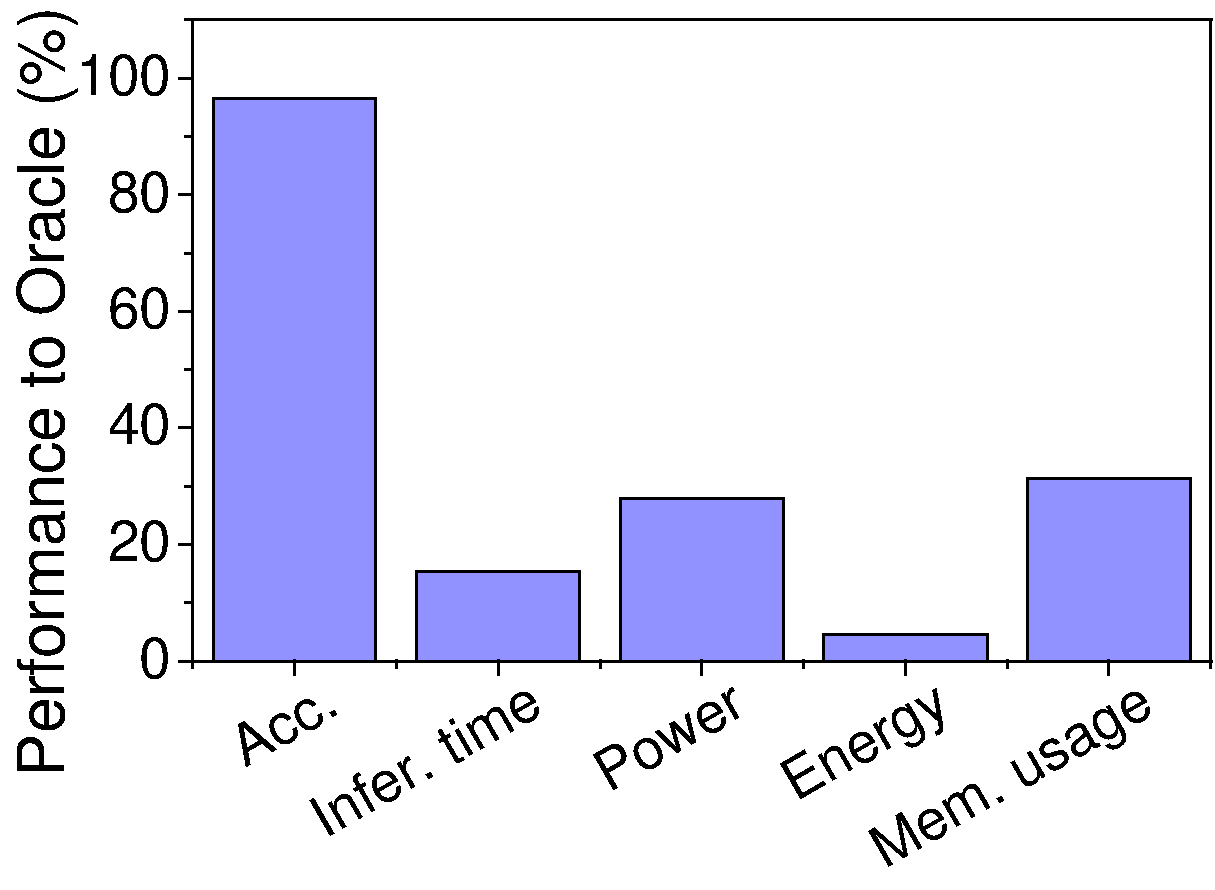
\includegraphics[width=0.2\textwidth]{figure/quan_oracle.pdf}}
%\hfill
%\subfloat[][\pruning]{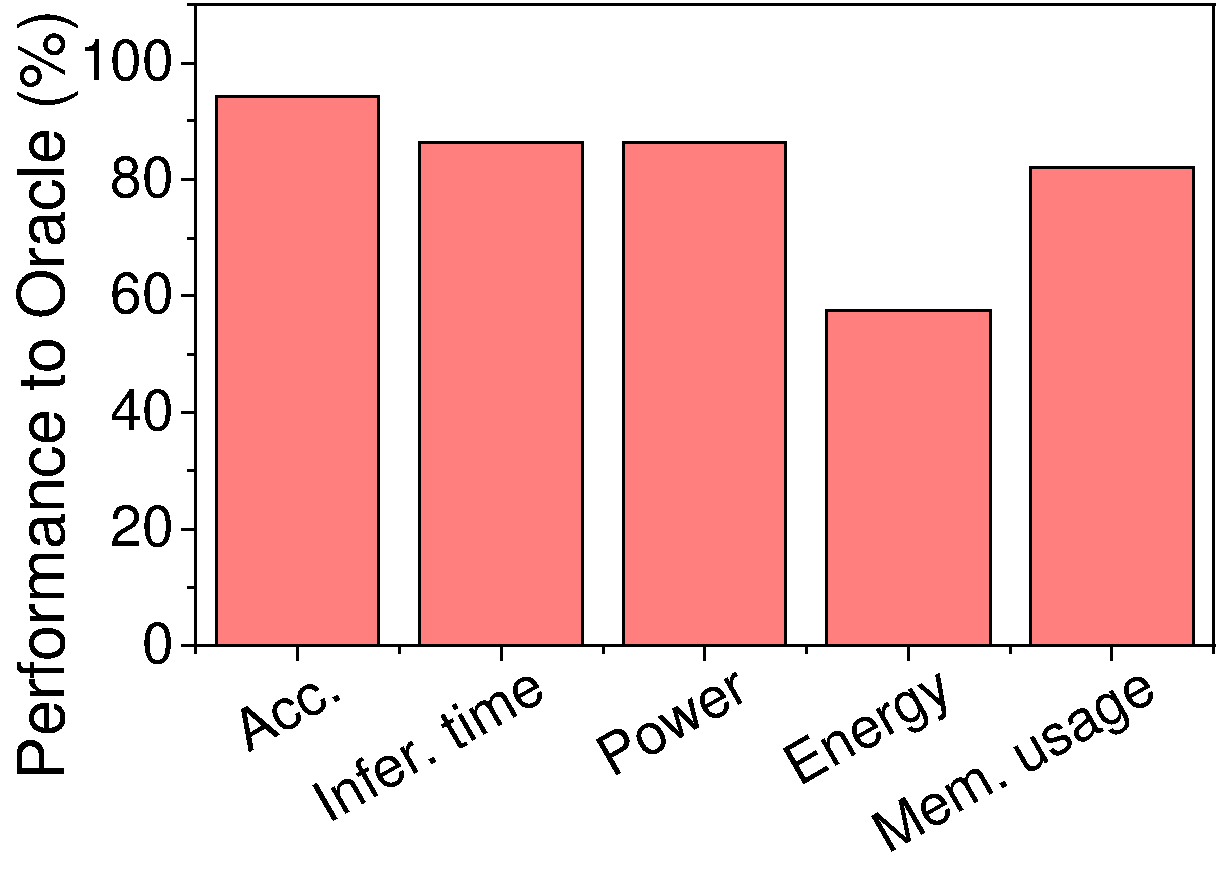
\includegraphics[width=0.2\textwidth]{figure/prun_oracle.pdf}}
%\hfill

%\caption{Compare to ideal 8-bit representation for \quantization (a) and \pruning (b).} \label{fig:oracle}
%\end{figure}
%For \quantization, we use the 8-bit representation as the ideal compressed model which 
%offers an affordable accuracy after quantization.
%Figure~\ref{fig:oracle}  compares our compressed models to the ideal 8-bit data quantization conditions.
%We can see that,  the accuracy of our 8-bit representation almost achieves the ideal value, on the
% less than 10\%. 
%Figure~\ref{fig:oracle} b presents the how close our pruned models to the theoretically perfect models. 
%As we can
%see from this figure, our pruned models achieve above 80\% , and the energy consumption also achieves 58\%.

\subsection{Combining Pruning and Quantization\label{sec:combin}}

\begin{figure*}[!t]
\centering
\subfloat[][Model size]{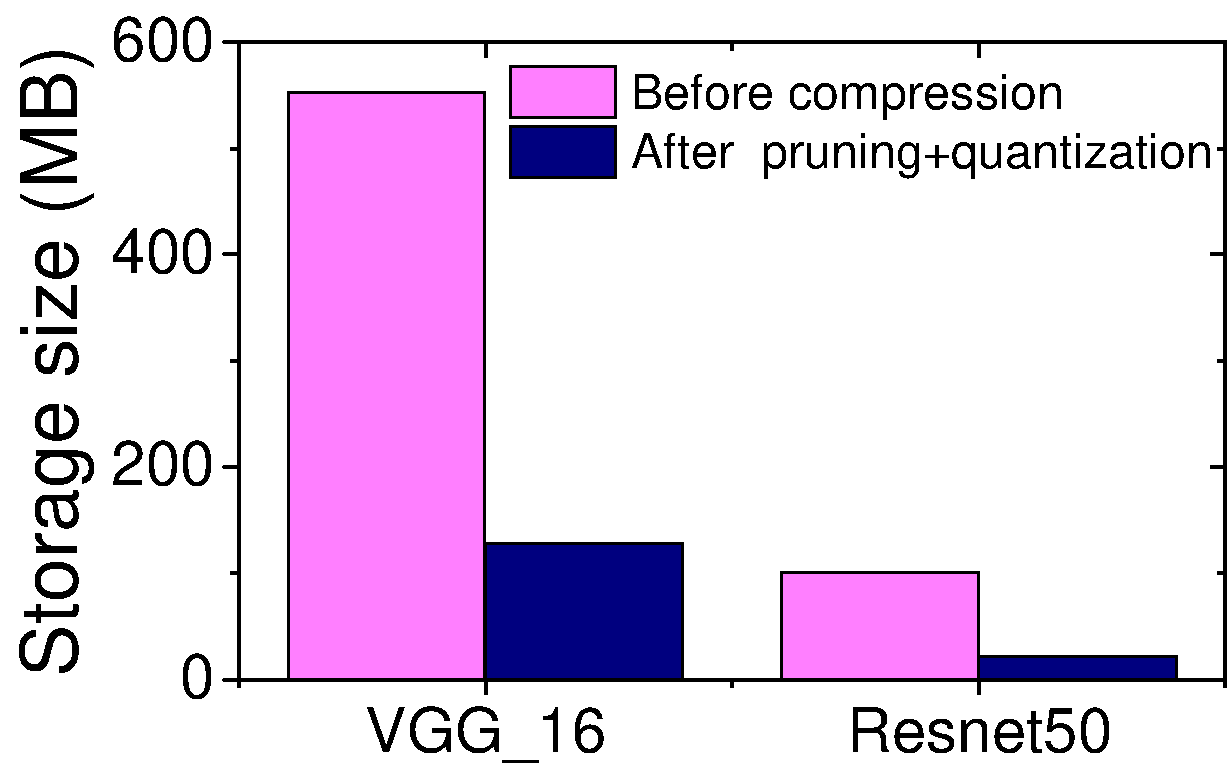
\includegraphics[width=0.24\textwidth]{figure/q_p_size.pdf}}
\hfill
\subfloat[][Inference time]{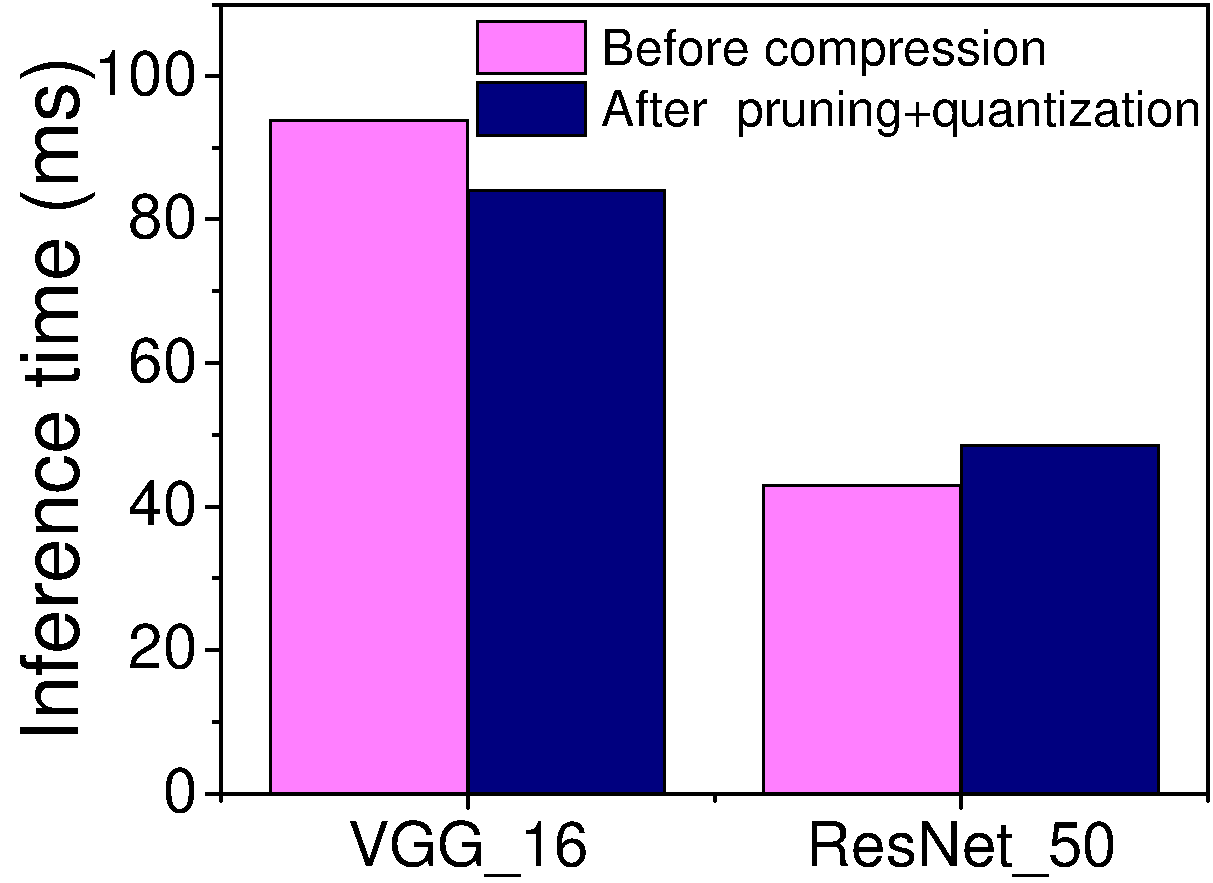
\includegraphics[width=0.24\textwidth]{figure/q_p_time.pdf}}
\hfill
\subfloat[][Energy consumption]{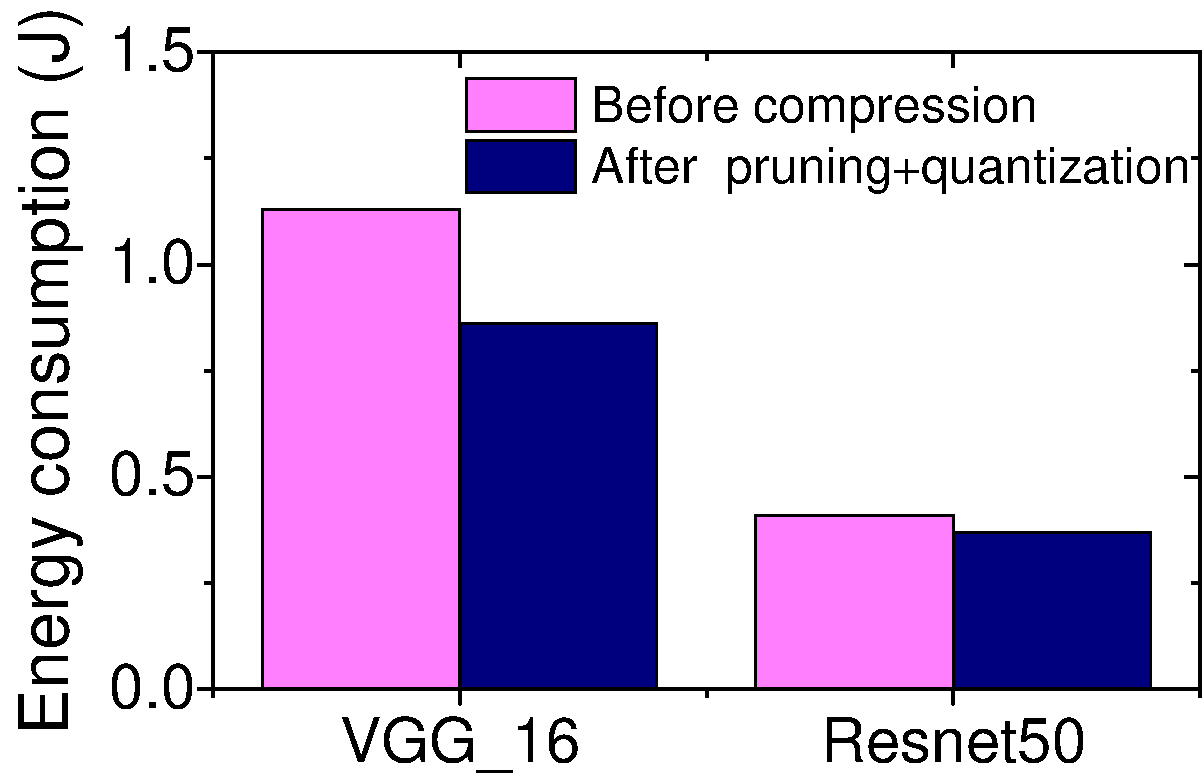
\includegraphics[width=0.23\textwidth]{figure/q_p_energy.pdf}}
\hfill
\subfloat[][Accuracy]{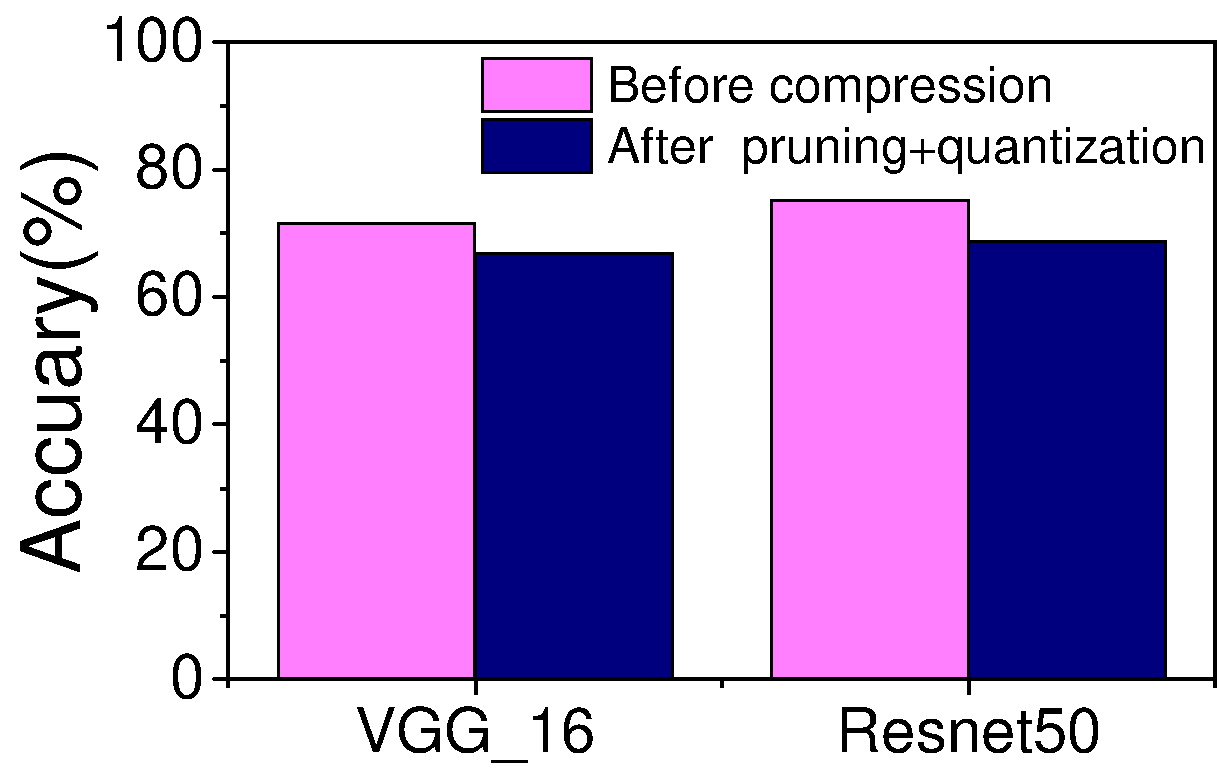
\includegraphics[width=0.24\textwidth]{figure/q_p_acc.pdf}}
\hfill
\caption{The achieved model size (a) inference time (b) energy consumption (c) and accuracy (d) before and after applying \quantization and \pruning.
}
\vspace{-5mm}
\label{fig:combine}
\end{figure*}

So far we have evaluated \pruning and \quantization in isolation. An natural question to ask is: ``Is it worthwhile to combine both
techniques?". Figure~\ref{fig:combine} shows the results by first applying a 8-bit \dquantization and then \pruning to \texttt{VGG\_16} and
\texttt{Resnet50}.


As can be seen from Figure~\ref{fig:combine}a, combining both compression techniques can significantly reduce the model storage size -- the
resulting models are 76\% smaller than the original ones; and there is little degradation in the top-1 prediction accuracy
(Figure~\ref{fig:combine}d) -- less than 7\%. From Figure~\ref{fig:combine}b, we see that the combination has positive impact on the
inference time for \texttt{VGG\_16} as the runtime overhead of \dquantization (see Section~\ref{sec:time}) can be amortized by \pruning.
The combination, however, leads to longer inference time for \texttt{Resnet50} due to the expensive de-quantization overhead as we have
explained. Because of the difference in inference time, there is less benefit in energy consumpation for \texttt{Resnet50} over
\texttt{VGG\_16} (Figure~\ref{fig:combine}c). This experiment shows that combining \pruning and \quantization can be beneficial, but it
depends on the neural network architecture and what to optimize for.
